% \documentclass[a4paper,12pt]{book}
\documentclass[11pt, twoside, openright]{thesis}

\usepackage{psl-cover}
\usepackage{lmodern}
\definecolor{maincolor}{RGB}{36, 56, 141}
\colorlet{secondarycolor}{violet}

\input{math_commands.tex}

% \usepackage[
% includehead,
% nomarginpar,
% includefoot,
% textheight=24cm,
% footskip=1.5cm]{geometry}
\geometry{
includehead,
nomarginpar,
includefoot,
textheight=24cm,
footskip=1.5cm}
\usepackage[utf8]{inputenc}
\usepackage[margin=0.5cm,labelfont=bf]{caption}
\usepackage{subcaption}
\usepackage{graphicx}
\usepackage[style=authoryear-comp,
backref=true
]{biblatex}

\DefineBibliographyStrings{english}{%
  backrefpage = {Cited on page},% originally "cited on page"
  backrefpages = {Cited on pages},% originally "cited on pages"
}

\usepackage{setspace}

\doublespacing

\usepackage{bold-extra}
\usepackage{amsmath}
\usepackage{csquotes}
\usepackage{amssymb}
\usepackage{dsfont}
\usepackage{array}
\usepackage{tikz}
\usepackage{booktabs}
\usepackage{nameref}
\usepackage{mathtools}
\usepackage[stretch=10]{microtype}
\usepackage{acronym}
\usepackage{xcolor}
\usepackage{colortbl}
\usepackage{multirow}
\usepackage{xspace}
\usepackage{url}
\usepackage{xhfill}
\usepackage[version=4]{mhchem}
\usepackage{anyfontsize}
\newcommand{\eg}{e.g.,\xspace}
\newcommand{\bigeg}{E.g.,\xspace}
\newcommand{\etal}{\textit{et~al.\xspace}}
\newcommand{\etc}{etc.\@\xspace}
\newcommand{\ie}{i.e.,\xspace}
\newcommand{\bigie}{I.e.,\xspace}
\usepackage[symbol]{footmisc}

\usepackage{fancyhdr}
% Please leave these options as they are
\usepackage{hyperref}
\usepackage{cleveref}
\hypersetup{
    colorlinks=true,
    linkcolor=red,
    filecolor=magenta,
    urlcolor=blue,
    citecolor=purple,
    pdftitle={Overleaf Example},
    pdfpagemode=FullScreen,
    }


\def\smtt#1{\texttt{\textsc{#1}}}
\acrodef{WADE}[WADE]{Weighted Average Data Efficiency}
\acrodef{RNN}[RNN]{recurrent neural network}
\newacro{ESN}{echo-state network}
\newacro{DS}{dynamical system}
\newacro{CA}{cellular automaton}
\newacroplural{CA}[CA]{Cellular automata}
\newacro{ECA}{elementary cellular automaton}
\newacroplural{ECA}[ECA]{Elementary cellular automata}

\newacro{NCA}{neural cellular automaton}
\newacroplural{NCA}[NCA]{neural cellular automata}
\newacro{CNN}{convolutional neural network}
\newacro{RBN}{random boolean network}
\newacro{OEE}{open-ended evolution}
\newacro{AC}{artificial chemistry}
\newacroplural{AC}[AC]{artificial chemistries}
\newacro{NS}{novelty search}
\newacro{RC}{reservoir computing}

\AtBeginEnvironment{thebibliography}{\linespread{1}\selectfont}

\urldef\projecturl\url{https://hugocisneros.com/ALIFE-Paper-2020/}

\title{Unsupervised Learning in Complex Systems}
\institute{L'École normale supérieure de Paris}
\doctoralschool{Sciences Mathématiques de\\ Paris Centre}{386}
\specialty{Informatique}
\author{Hugo Cisneros}
\date{2022}

\jurymember{1}{Name 1}{Université 1}{Président du jury}
\jurymember{2}{Name 1}{Université 1}{Rapporteur}
\jurymember{3}{Name 2}{Université 2}{Rapporteur}
\jurymember{4}{Name 3}{Université 3}{Examinatrice}
\jurymember{5}{Josef Sivic}{École Normale Supérieure, Inria\\CIIRC, Czech Technical University}{Directeur de thèse}
\jurymember{6}{Tomas Mikolov}{CIIRC, Czech Technical University}{Directeur de thèse}

\frabstract{
%Résumé

}

\enabstract{
%Abstract
  The goal of this thesis is to develop systems that can learn without
  supervision and develop autonomously while becoming more complex over time.
  Complex systems are a framework for studying learning and adaptation in
  natural systems. They have the potential to exhibit growth of complexity. In
  this thesis, we propose using complex systems as a framework for studying
  these phenomena and develop methods to study the computations that take place
  in these systems. Our ultimate goal is to create learning algorithms that
  require limited to no supervision, allowing for greater flexibility and
  adaptability in a wide range of applications. By understanding the fundamental
  principles of learning in complex systems, we hope to advance our ability to
  design and implement effective learning algorithms in the future. The thesis
  makes the following key contributions: the development of a general complexity
  metric that we apply to search for complex systems that exhibit growth of
  complexity, the introduction of a coarse-graining method to study computations
  in large-scale complex systems, and the development of a metric for learning
  efficiency as well benchmark dataset for evaluating the speed of learning
  algorithms. Our approach offers a promising new direction for research in this
  area and has the potential to advance our understanding of learning and
  adaptation in natural and artificial systems, leading to the development of
  more effective and efficient learning algorithms in the future. }

\frkeywords{Apprentissage automatique {\Large\color{maincolor}$\star$} Intelligence
  artificielle {\Large\color{maincolor}$\star$} Systèmes complexes
  {\Large\color{maincolor}$\star$} Complexité}

\enkeywords{ Machine learning {\Large\color{maincolor}$\star$} Artificial
  Intelligence {\Large\color{maincolor}$\star$} Complex systems
  {\Large\color{maincolor}$\star$} Complexity}

\addbibresource{main.bib}


% For the printable version
% \printversiontrue

\ifprintversion
\else
\geometry{
left=1.25in,
right=1.25in,
}
\fi

% \begin{document}
% \maketitle
\begin{document}
\frontmatter
\hypersetup{pageanchor=false}
\maketitle
\hypersetup{pageanchor=true}
% \dominitoc

% \begin{dedication}
%   Dedication...
% \end{dedication}
% \tableofcontents

\ifprintversion
    \setboolean{@twoside}{true}
    \pagestyle{fancy}
    \fancyhead{} % clear all header fields
    \fancyhead[ER,OL]{\footnotesize \rightmark} \fancyhead[EL,OR]{\thepage}
    \fancyfoot{} % clear all footer fields
    \fancyfoot[C]{---\quad \textbf{H. Cisneros: Unsupervised Learning in
        Complex Systems}\quad ---}
\else
    \setboolean{@twoside}{false}
    \pagestyle{fancy}
    \fancyhead{} % clear all header fields
    \fancyhead[R]{\footnotesize \rightmark} \fancyhead[L]{\thepage}
    \fancyfoot{} % clear all footer fields
    \fancyfoot[C]{---\quad \textbf{H. Cisneros: Unsupervised Learning in
        Complex Systems}\quad ---}
\fi

\cleardoublepage
\chapter*{Résumé}
\addstarredchapter{Résumé}
\thefrabstract{}
\vfill
\thefrkeywords{}
\cleardoublepage
\chapter*{Abstract}
\addstarredchapter{Abstract}
\theenabstract{}
\vfill
\theenkeywords{}

\cleardoublepage
\chapter*{Acknowledgments}
\addstarredchapter{Acknowledgments}
% Acknowledgments

\cleardoublepage
\hypertarget{contents}{}
\tableofcontents

\mainmatter
\chapter{Introduction}

\section{Goal}

\subsection{Unsupervised learning}

\subsection{Complex systems}

\subsection{Cellular automata}

\section{Motivation}
\section{Challenges}

\chapter{Background}
\label{cha:background}

\section{Cellular automata}

\Acp{CA} were originally proposed by Stanislaw Ulam and John Von
Neumann in the 1940s as a model of the growth of crystals and an attempt at
constructing a self-replicating system \cite{von_neumann_theory_1966}.

It is usually defined on a regular lattice in one or two dimension. Each of its
components is called a cell, and can be in a state $k \in \mathcal{S}$. A neighborhood
function $\boldsymbol{N}$ is defined which associates each cell with its
neighbors on the lattice.

In general, a \ac{CA} can be constructed on any space
$\mathcal{L}$ where such a function can be defined.
In practice, regular finite or infinite grids are chosen, $\mathcal{L} \subset \mathbb{Z}$ or
$\mathcal{L} \subset \mathbb{Z}^{2}$. For example, the grid could be a 1-dimensional torus with 10 cells,
that is $\mathcal{L}_{{T_{10}}} = \{1, 2, \ldots, 10 \}$.

The neighborhood function has the form

\begin{equation}
  \begin{aligned}
\boldsymbol{N} :\quad & \mathcal{L} \rightarrow \mathcal{L}^{s}\\
&c \mapsto [c_{i}]_{i=1}^{s}
  \end{aligned}
\end{equation}
,

where the returned value is a finite number of cells, the neighbors of cell $c$.
For the torus $\mathcal{L}_{T_{10}}$ above, we can define the neighbors to be the cell
itself and the two immediately adjacent cells. This type of 1D neighborhood is
illustrated on Figure \ref{fig:1d_neigh}. It corresponds to the following
neighborhood function
\begin{equation}
  \begin{aligned}
\boldsymbol{N} :\quad & \mathcal{L}_{T_{10}} \rightarrow \mathcal{L}_{T_{10}}^{3} \\
&\boldsymbol{N}(c) = \begin{cases}
                      [c - 1, c, c + 1],& \text{if}\quad c \in \{2,\ldots , 9\}\\
                       [10, 1, 2], & \text{if} \quad c = 1 \\
                       [9, 10, 1], & \text{if} \quad c = 10. \\
                    \end{cases}
  \end{aligned}
\end{equation}

On two dimensional grids, there are multiple ways to define the neighborhood.
Some common examples are the Moore neighborhood and the Von Neumann neighborhood.

\begin{figure}[htbp]
  \centering
  \begin{subfigure}[c]{.3\linewidth}
    \centering
    \includegraphics[width=\linewidth]{figures/1d_neigh}
    \caption{Standard 1D \ac{CA} neighborhood}
    \label{fig:1d_neigh}
  \end{subfigure}
  \begin{subfigure}[c]{.3\linewidth}
    \centering
    \includegraphics[width=\linewidth]{figures/moore}
    \caption{Moore neighborhood}
    \label{fig:moore}
  \end{subfigure}
  \begin{subfigure}[c]{.3\linewidth}
    \centering
    \includegraphics[width=\linewidth]{figures/von_neumann}
    \caption{Von Neumann neighborhood}
    \label{fig:von_neumann}
  \end{subfigure}

  \caption{Illustration of commonly used neighborhoods for 1D and 2D cellular automata.}
  \label{fig:neighborhoods}
\end{figure}


An update rule $\boldsymbol{\Phi}$ defines the new state of a cell as a function of its local
neighborhood. It is applied in parallel to all the cells.

A large number of variants of \acp{CA} have been constructed. We list some of
them here.

\subsection{Asynchronous cellular automata}
A cellular automaton is said to be asynchronous when its cells are not all
updated in parallel at each time step.

\subsection{Stochastic cellular automata}
A cellular automaton is said to be asynchronous when its cells are not all
updated in parallel at each time step.

\subsection{Discrete}
\subsection{Continuous}

\section{Reservoir computing}

\chapter{Literature Review}
\label{cha:literature-review}

\section{Computing with complex systems}

\chapter{Measuring complexity in evolving complex systems}
\label{cha:meas-compl-evolv}

In this chapter, we propose an approach for measuring growth of complexity of
emerging patterns in complex systems such as \acfp{CA}. We discuss several ways
in which a metric to measure complexity growth can be defined. This includes
approaches based on compression algorithms and artificial neural networks. We
believe that such a metric can be useful for designing systems that could exhibit
open-ended evolution, which itself might be a prerequisite for the development of
general artificial intelligence. We conduct experiments on 1D and 2D grid worlds
and demonstrate that using the proposed metric we can automatically construct
computational models with emerging properties similar to those found in
Conway's Game of Life, as well as many other emergent phenomena. Interestingly,
some of the patterns we observe resemble forms of artificial life 
\ref{langtonEditorIntroduction1993}. We test our
metric of structural complexity growth on cellular automata, but it can also be
applied to a wide range of complex systems.

\section{Introduction}
Recent advances in machine learning and deep learning have had success in
reproducing some very complex feats traditionally thought to be only achievable
by living beings. However, making these systems adaptable and capable of
developing and evolving on their own remains a challenge that could be crucial to eventually developing AI with general learning capabilities (for example, as
is further discussed in \parencite{mikolovRoadmapMachineIntelligence2018}).
Building systems that mimic some key aspects of the behavior of existing
intelligent organisms (such as the ability to evolve, improve, adapt, etc.)
might represent a promising path. Intelligent organisms --- for example, human beings but
also most living organisms if we consider a broad definition of intelligence ---
are a form of spontaneously occurring, ever evolving complex systems that
exhibit these kinds of properties
\parencite{bookerPerspectivesAdaptationNatural2004}. The ability to sustain
open-ended evolution appears to be a requirement in order to enable the emergence of
arbitrarily complex adaptive systems.

Although a rigorous attempt at defining intelligence or life is beyond the scope
of this work, we assume that a system we might identify as evolving, with the
potential of developing intelligence, should have the property of
self-preservation and the ability to grow in complexity over time. These
properties can be observed in living organisms
\parencite{bookerPerspectivesAdaptationNatural2004} and should also be part of
computational models that aim to mimic them.

To recognize self-preservation and growth in complexity, one should be able to
detect emerging macro-structures composed of smaller elementary components. For
the purpose of obtaining computational models that grow in complexity over time,
one should also be able to determine the amount of complexity these systems
contain. In this chapter, we propose and discuss several ways of estimating the
complexity and detecting the presence of emerging and stable patterns in complex
systems such as cellular automata. We show that such metrics are useful when
searching the space of cellular automata with the objective of finding those
that seem to evolve over time.

\section{Related work}

\subsection{Artificial life and open-ended evolution}

Several works have attempted to artificially create open-ended evolution. A
nonexhaustive list of some well-known systems include Tierra
\parencite{srayApproachSynthesisLife1991}, Sims
\parencite{simsEvolvingVirtualCreatures1994}, Avida
\parencite{ofriaAvidaSoftwarePlatform2004}, Polyworld
\parencite{yaegerComputationalGeneticsPhysiology1994}, Geb
\parencite{channonImprovingStillPassing2003}, Division Blocks
\parencite{spectorDivisionBlocksOpenended2007} and Chromaria
\parencite{sorosIdentifyingNecessaryConditions2014}. Designs that focus on an objective and make use of reinforcement learning methods to drive evolution
are also being studied, e.g. in
\parencite{pathakLearningControlSelfAssembling2019}. Most of these simulated
``worlds'' have had some success in reproducing key aspects of evolving
artificial life, enabling the emergence of complex behavior from simple
organisms. However, they still work within constrained simulated environments
and usually consider organisms composed of elementary building blocks, while
they do not work outside of this usually very constrained framework. The divergent
and creative evolutionary process could be happening at a much lower conceptual
level with fewer assumptions. For this reason, we consider cellular automata in
the rest of the chapter because they rely on very few assumptions while
offering a very large expressive power and a potentially wide range of behaviors
that can be discovered. However, the metrics defined in this work have the
potential to be applied to other types of complex systems, as discussed in
Section~\ref{sec:conclusion}.

\subsection{Cellular automata}

Cellular automata are very simple systems, usually defined in one or two
dimensions, composed of cells that can be in a set of states. The cells are
updated in discrete time steps using a transition table that defines the next
state of a cell given the states of its neighbors. They were originally proposed
by Stanislaw Ulam and studied by Von Neumann
\parencite{vonneumannTheorySelfreproducingAutomata1966}, who was interested in
designing a computational system that can self-reproduce itself in a nontrivial
way. The trivial self-reproducing patterns were then those that do not have the
potential to evolve, for example the growth of crystals.

Stephen Wolfram later took a more bottom-up approach, beginning with the study
of simple 1D binary cellular automata (CA), and identifying four qualitative
classes of cellular automaton behavior
\parencite{wolframUniversalityComplexityCellular1984}:

\begin{description}
\item[Class 1] evolves to a homogeneous state.
\item[Class 2] evolves to simple periodic patterns.
\item[Class 3] yields aperiodic disordered patterns.
\item[Class 4] produces complex aperiodic and localized structures, including
  propagating structures.
\end{description}

Wolfram and his colleagues also studied 2D CA using tools from information
theory and dynamical systems theory, describing the global properties of these
systems in terms of entropies and Lyapunov exponents
\parencite{packardTwodimensionalCellularAutomata1985}.

Christopher Langton and colleagues also studied CA dynamics
\parencite{liTransitionPhenomenaCellular1990} --- e.g. using the $\lambda$ parameter
\parencite{langtonComputationEdgeChaos1990} --- and designed a self-replicating
pattern much simpler than Von Neumann's
\parencite{langtonSelfreproductionCellularAutomata1984}, now known as Langton
loops. The main issues with his system and Von Neumann's universal replicator is
the fact that they are very fragile and based on a large amount of human design.
As a consequence, although they self-replicate, they cannot increase in
complexity and are not robust to perturbations or unexpected interactions with
the environment.

A genetic algorithm-based search for spontaneously occurring self-replicating
patterns in 2D cellular automata with several states was undertaken in
\parencite{bilottaARTIFICIALMICROWORLDSPART2011} using entropy measures of the
frequency distribution of $3\times 3$ patterns.

\subsection{Compression and complexity}
Compression has often been used as a measure of complexity. Lempel and Ziv have
introduced in \parencite{lempelComplexityFiniteSequences1976} the now widespread
Lempel-Ziv (LZ) algorithm as a method for measuring the complexity of a
sequence. By constructing back-references to previous parts of a string, the LZ
algorithm is capable of taking advantage of duplicate patterns in the input to
reduce its size. The DEFLATE algorithm that we use in the following section
combines LZ with Huffman coding for efficient representation of the symbols
obtained after the first step. It is one of the most widespread compression
algorithms and is, for instance, used in gzip and PNG file compression standards.

The PAQ compression algorithm series \parencite{mahoneyFastTextCompression2000}
is an ensemble of compression algorithms initially developed by Matt Mahoney
with state-of-the-art compression ratio on several compression benchmarks.
Better compression of an input means a better approximation of the minimum
description length and implicit understanding of more of the underlying patterns
in input data. The usefulness of a better compressor is that it can detect much
more complex and intricate patterns that aren't simple repetitions of previous
patterns.

In \parencite{zenilCompressionBasedInvestigationDynamical2010}, H. Zenil
investigates the effects of a compression-based metric to classify cellular
automata and observes that it results in a partitioning of the space of 1D CA
into several clusters that match Wolfram's classes of automata. He also used
this approach in the output of simple Turing machines and some 1D automata with
more than two states and larger neighborhoods. Extensions of this work include
asymptotic sensitivity analysis of compressed length for input
configurations of growing complexity, as introduced in
\parencite{zenilAsymptoticBehaviorRatios2013,
  zenilWhatNatureLikeComputation2014}.

Additionally, image decompression time as an approximation of Bennet's logical
depth \parencite{bennettLogicalDepthPhysical1995,
  zenilImageCharacterizationClassification2012} and the output distribution of
simple Turing machines combined with block decomposition of CA to approximate
their algorithmic complexity have also been investigated
\parencite{zenilTwodimensionalKolmogorovComplexity2015,
  soler-toscanoCalculatingKolmogorovComplexity2014}. However, the possible
extent to which such measures of complexity could be applied to more complex
automata and other complex systems has not yet been extensively studied. For a
review of several measures of complexity and their applications, see
\parencite{grassbergerRandomnessInformationComplexity1989}.

\section{Compression-based metric}\label{sec:compr-based-metr}

A cellular automaton of size $n$ in 1D can be represented at time $t$ by its
grid-state $S^{(t)} = \{c_1^{(t)}, ..., c_n^{(t)}\}$ where each $c_i$ (also
called a cell) can take one of $k$ possible values (representing the possible
states) and a transition rule $\phi$. The transition rule is defined with
respect to a neighborhood radius $r$ with the mapping $\phi(c^{(t)}_{i-r}, ...,
c^{(t)}_i ..., c^{(t)}_{i+r} ) = c^{(t+1)}_i$ that maps $\{1, ..., k\}^{2r+1}$
to $\{1, ..., k\}$. The quantity $2r + 1$ corresponds to the number of
cells taken into account to calculate the next state of a cell, namely the
cell itself and $r$ neighboring cells in both directions.

Simulating a CA amounts to the recursive application of this mapping $\phi$ to
an initial state $S^{(0)} = \{c_1^{(0)}, ..., c_n^{(0)}\}$.

In the rest of the chapter, we consider cyclic boundary conditions for the
automata, meaning that the indices $i-r, ..., i+r$ above are taken modulo $n$
the size of the automaton in 1D. Boundary conditions can have some effect on a
CA's evolution, but cyclic boundaries have been empirically observed to have
limited effect on the complexity of automata in 1D
\parencite{luvalleEffectsBoundaryConditions2019}.

The definition given in the equation above can be extended to higher dimensional
automata by modifying the neighborhood and the definition of $\phi$. A 2D
neighborhood of radius 1 can be defined as the 3 by 3 square around the center
cell --- also called the Moore neighborhood --- or by only considering the four
immediate horizontal and vertical neighbors of the center cell --- the Von Neumann
neighborhood.

Elementary cellular automata (ECA) are 1D CA with $k = 2$ and $r = 1$. There are
$2^3$ elements in $\{1, ..., k\}^{2r+1}$ and $2^{2^3} = 256$ possible different
set transition rules that are often compactly represented as a binary string
with 8 bits. The relatively low number of rules of this type makes it possible
to appreciate the performance of a metric and compare it with others.

We define the compressed length $C$ of a 1D cellular automaton at time $t$ as
\begin{align}
  C(S^{T}) = \text{length}\left(\texttt{comp}(c_1\ ||\ c_2\ ||\ ...\ c_n)\right)
\end{align}

where $||$ denotes the string concatenation operator and the cells $c_i$ are
implicitly converted into string characters (with one symbol per unique state).
\texttt{comp} is a compression algorithm that takes a string as input and
outputs a compressed string, and length is the operator that returns the length
of an input string.

Similarly to \parencite{kowaliwMeasuresComplexityArtificial2008,
  zenilCompressionBasedInvestigationDynamical2010}, we use zlib’s C
implementation of DEFLATE to compress the final state of the automaton. If we
apply the above metric to the 256 ECA run for 512 timesteps and initialized with
one activated cell in the middle, we obtain the plot of
Figure~\ref{subfig:comp_scores}. This example is re-used in the rest of the
chapter as a way to easily visualize and check that the defined complexity
measures are coherent with one another. The colors on
Figure~\ref{subfig:comp_scores} were obtained with a KMeans clustering algorithm
applied on the compressed length of the automata states.

\begin{figure}[tbp]
  \begin{subfigure}[b]{.47\linewidth}
    \centering
    \includegraphics[width=\linewidth]{figures/complex_eca}
    \caption{6 highest scoring automata. Only the first 30 timesteps are shown
      for readability.}
    \label{subfig:highest_6}
  \end{subfigure}
  \hspace{10pt}
  \begin{subfigure}[b]{.47\linewidth}
    \centering
    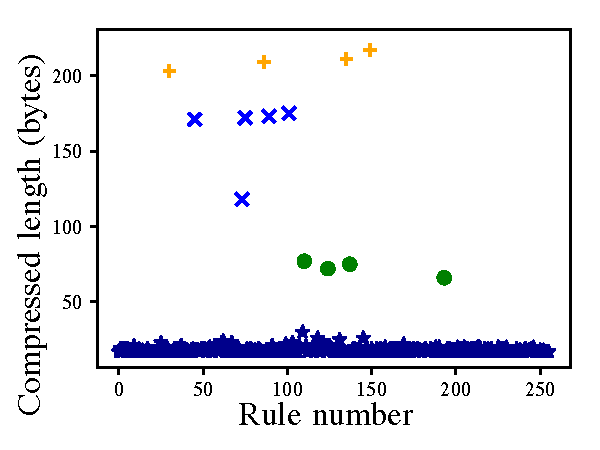
\includegraphics[width=\linewidth]{figures/one}
    \caption{All 256 compressed length scores.}
    \label{subfig:comp_scores}
  \end{subfigure}
  \caption{Compression-based metric on 1D ECA. \ref{subfig:highest_6} represents
    the 1D ECA evolution with each line being the state of the automaton at a
    given timestep, starting from a single cell set to 1. Cells which are in
    state 1 are represented in black and cells in state 0 are represented in
    white. Time increases downwards. Figure~\ref{subfig:comp_scores} represents
    the compressed length of the 256 ECA rules, with different marker and colors
    corresponding to the obtained KMeans clusters.}

  \label{fig:comp_eca}
\end{figure}


As visible on Figure~\ref{subfig:comp_scores}, rules are clearly separated into
several clusters that turn out to match Wolfram’s classification of ECA. Class 3
behavior can be found at the top of the plot (highest compressed length, orange
and blue clusters), Class 1 and 2 are clearly separated at the bottom part (not
detailed here) and Class 4 rules (colored in green) lie in between the other
types of behavior. The 6 highest scoring rules are shown on
Figure~\ref{subfig:highest_6} and correspond to Class 3 behavior in Wolfram's
classification. Among the classes of behavior, some sub-clusters can be found
that correspond to similarly behaving rules.

Ultimately, the theoretical goal of using compression algorithms is to approach
the theoretical minimum description length of the input
\parencite{grunwaldMinimumDescriptionLength2007}. For very regular inputs, this
length should be relatively small and inversely for random inputs. However, gzip
and PAQ are crude approximations of the minimum description length, and may only
approach it in a given context. As an example, compressing text data (a task
often performed with gzip in practice) is much more efficient with a language
model that can assign a very low probability to non grammatically correct
sentences. The Kolmogorov complexity
\parencite{kolmogorovThreeApproachesQuantitative1968} of a cellular automaton is
upper bounded by a value that is independent of the chosen rule, as it is
entirely determined by the transition table, the grid size, initial
configuration and number of steps.

\section{Predictor-based metric}

One obvious limit of using compression length as a proxy for complexity is the
fact that interesting systems mostly have intermediate compressed length.
Compressed length increases with the amount of disorder in the string being
compressed. Therefore, extreme lengths correspond either to systems that do not
increase in complexity on the lower end of the spectrum, or systems that produce
a maximal amount of disorder on the higher end. Neither of them have the
potential to create interesting behavior and increase in complexity.
Intermediate values of compressed length are also hard to interpret, since
average lengths might either correspond to interesting rules or slowly growing
disordered systems.

To cope with this limitation, one should also take into account the dynamics of
complexity, that is how the system builds on its complexity at a given time as
it keeps evolving, while retaining some of the structures it had acquired
earlier. Compression leverages the amount of repetitions in inputs to further
compress and this may also be used as an estimate of structure overlap, as
explained in the following section.

\subsection{Joint compression}\label{sec:joint-compression}

As a way to both measure the complexity and the amount of overlap between two
automata states apart in time, we define a joint compressed length metric for a
delay $\tau$ as
\begin{align}
  C'\left(S^{(T + \tau)}, S^{(T)}\right) =
  C\left(S^{(T)}\ ||\ S^{(T + \tau)}\right)
\end{align}
where $||$ represents the concatenation operator. This quantity is simply the
compressed length of a pair of global states --- defined at the beginning of
\ref{sec:compr-based-metr}, represented by the letter $S$ --- at two timesteps
separated by a delay $\tau$. In 1D, concatenation means chaining the two string
representations before compressing, and in 2D we can chain two flattened
representations of the 2D grid. This introduces several issues which we discuss
in Section~\ref{sec:count-based-pred}.

To quantify the amount of overlap between the two global states, we can compute
the ratio of this joint compressed length with the sum of the two compressed
lengths $C(S^t)$ and $C(S^{t-\tau})$, thereby forming the joint compression
score
\begin{align}
  \mu = \dfrac{C\left( S^t \right) +
  C\left( S^{t - \tau} \right)}{C'\left( S^t, S^{t - \tau} \right)}
\end{align}
defined for an automaton $S$, time $t$ and delay $\tau$.

This metric is based on the intuition that if patterns occur at step $T - \tau$
of the automaton's evolution and are still present at step $T$, the joint
compressed length will be lower than the sum of the two compressed length. The
idea is illustrated in Figure~\ref{fig:joint_schema}, where it is pointed out
that a stable moving structure (sometimes called \emph{glider} or
\emph{spaceships} in Game of Life) will yield lower joint compressed lengths.
This also applies to structures that self-replicate, grow from a stable seed or
maintain the presence of some sub-structures. Bigger structures yield a higher
compression gain.

\begin{figure}[htbp]
  \centering
  \includegraphics[width=\linewidth]{figures/joint_comp_1d}
  \caption{Joint compression method illustration. If a structure persists
    through time, this will decrease the joint compressed length compared to the
    sum of compressed lengths. A persistent structure is circled in red.}
  \label{fig:joint_schema}
\end{figure}

Joint compression alone is not sufficient since it only selects rules that
either behave like identity or shift input because they maximize the
conservation of structures through time --- as illustrated in
Figure~\ref{fig:high_eca_joint}. However, one may combine the joint compression
score with another complexity measure to only select rules that exhibit some
disorder, or growth in complexity --- as Figure~\ref{fig:high_eca_joint+comp}
shows (the condition here was a threshold on the difference of compressed length
between initial and final states).

\begin{figure}[htbp]
  \centering
  \begin{subfigure}[b]{.45\linewidth}
    \centering
    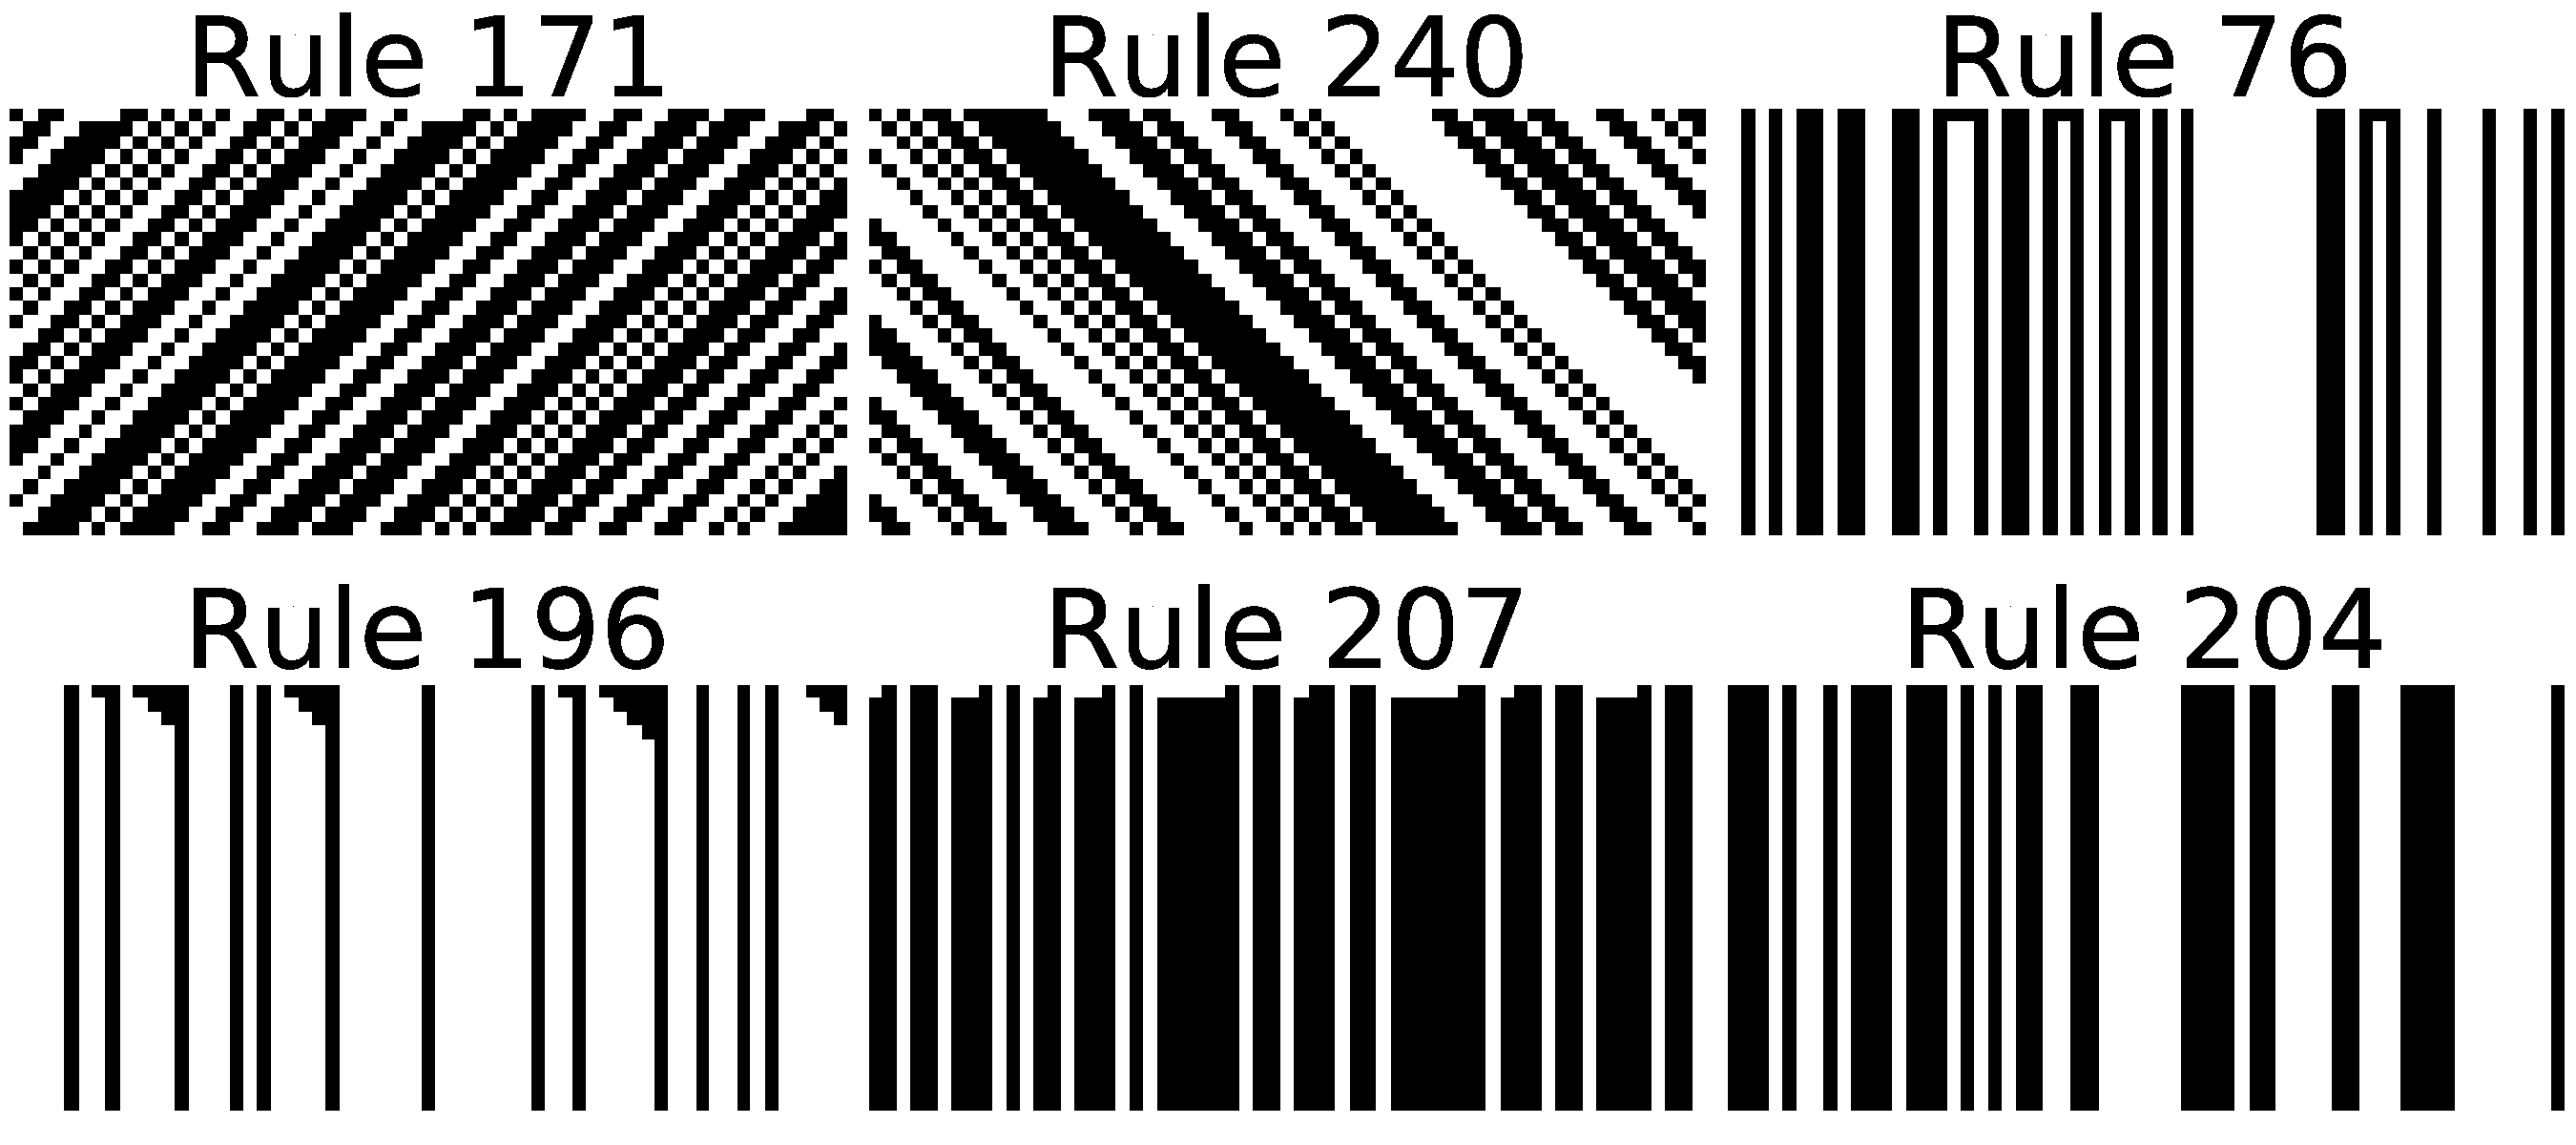
\includegraphics[width=\linewidth]{figures/high_eca_joint}
    \caption{Highest joint compression score among the 256 ECA.}
    \label{fig:high_eca_joint}
  \end{subfigure}
  \begin{subfigure}[b]{.45\linewidth}
    \centering
    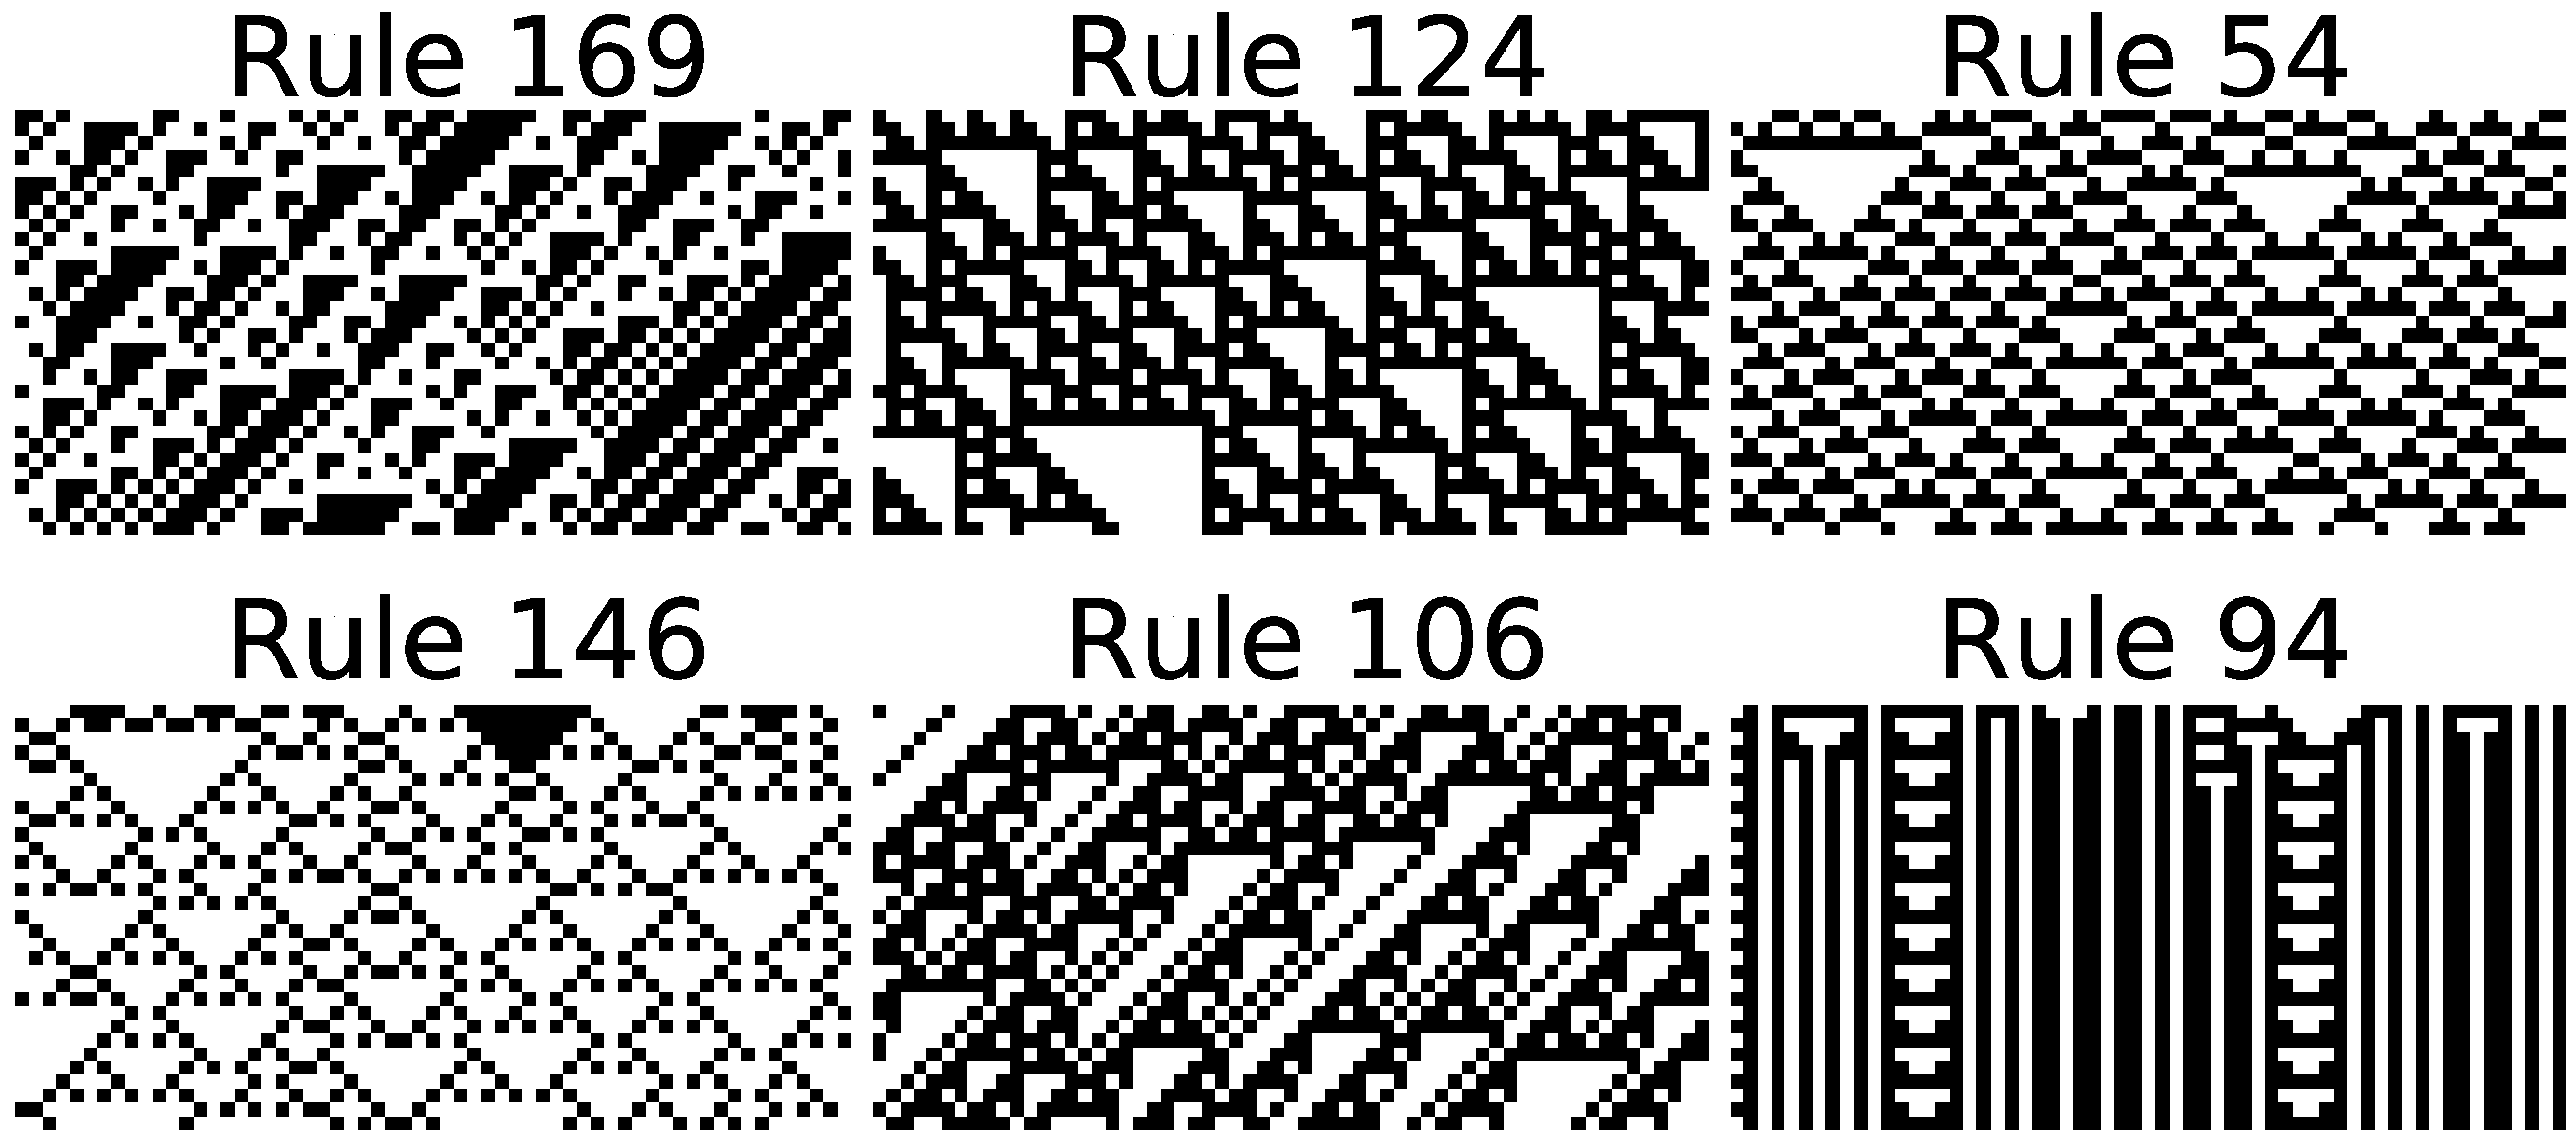
\includegraphics[width=\linewidth]{figures/high_eca_joint+comp}
    \caption{With condition on compressed length increase.}
    \label{fig:high_eca_joint+comp}
  \end{subfigure}

  \caption{Comparison of the raw joint compression score and the addition of a
    complexity increase condition. The high overlap in structures is not enough
    to get interesting rules a shown in \ref{fig:high_eca_joint}, but the
    addition of a complexity threshold allows to retrieve rules with complex but
    still structured behavior, as shown in \ref{fig:high_eca_joint+comp}.
    Figures are from the same slice of 60 cells over 30 timesteps taken from
    larger automata with random initial states. The top row corresponds to $t =
    0$ and time increases downwards.}
  \label{fig:joint_highest}
\end{figure}

\subsection{Count-based predictor}\label{sec:count-based-pred}

A major issue with the joint compression metric is the fact that it is designed
to compress a linear stream of data. This is not ideal when considering higher
dimensional automata. Larger sets of transformations have to be
considered such as translations, rotations, flips, etc. Theoretically this
should not be a problem for a good enough linear compression algorithm, but
hardware and software limitations make it impractical to work with existing
algorithms on higher dimensional structures --- with e.g DEFLATE's upper limit
on dictionary size.

These higher dimensional automata might be better at generating complex
dynamics, and the large size of their rule spaces makes it a challenge to
explore. There has been at least one attempt to deal with these higher
dimensional systems \parencite{zenilTwodimensionalKolmogorovComplexity2015} that lacks the scalability
to work with large inputs.

An alternative to the linear compression-based method presented above would be
to use compressors optimized for n-dimensional data (e.g. PNG compression for 2D
automata) to take advantage of spatial correlation for compressing. However,
these compressors are rare for higher dimensional data, and are usually
optimized for one type of input --- e.g. images with PNG.

Another way to tackle the problem is to use a prediction based approach to
compression. Similarly to methods described in
\parencite{schmidhuberSequentialNeuralText1996} and one of the first steps of the PAQ
compression algorithm \parencite{mahoneyFastTextCompression2000}, we learn a statistical model of
input data to predict the content of a cell given its immediate predecessors.
For compression, this is often followed by an encoding step --- using Huffman or
arithmetic coding --- that encodes data which contains the least information
(least ``surprising'' data) with the most compact representation. This approach
can also be related to the texture synthesis method described in
\parencite{efrosTextureSynthesisNonparametric1999}, where the authors learn a non parametric model to
predict the next pixel of a texture given a previously synthesized neighborhood.
Additionally, because we do not need the operation to be reversible as in regular
compression, it is not necessary to limit the prediction model to making
prediction with predecessors only.

For a global state $S = (c_{1}, ... c_i, ..., c_{n})$, the neighborhood of cell
$i$ with radius $r$, denoted $n_{r,i}$ is defined as the tuple $n_{r,i} =
(c_{i-r}, ... c_{i-1}, c_{i+1} ..., c_{i+r})$ --- without the middle cell. The
goal of this method is to estimate the conditional probability distribution $p(s
| n_r)$ of the middle states at timestep $T$ given a neighborhood of radius $r$.
Assuming cell states given their neighborhood can be modeled by mutually
independent random variables, the log-probability of global state $S^{(T)}$ is
written
\begin{align}
  \log p(S^{(T)}) = \log \prod_{i=1}^N p(c_i | n_{r,i})  =
  \sum_{i=1}^N \log  p(c_i | n_{r,i})
\end{align}

If the automaton has a very ordered behavior, a model will predict with high
confidence the state of the middle cell given a particular neighborhood. On the
other hand, in the presence of maximal disorder, the middle cell will have an
equal probability of being in every state no matter the neighborhood. In the
latter case, a predictive model minimizing $-\log p(S^{(T)})$ would yield a high
negative log-probability.

A simple possible predictor for such purpose is a large lookup table that maps
all visited neighborhoods to a probability distribution over the states that the
middle cell can be in. State distributions for each neighborhood are obtained by
measuring the frequency of cell states given some observed neighborhoods. We
denote by $\Lambda$ this lookup table, defined for a window of radius $r$, which
maps all possible neighborhoods of size $2r + 1$ (ignoring the middle cell) to a
set of probabilities $p$ over the possible states $\{s_1, ..., s_n\}$, and $p$
can be written $[p_{s_1}, p_{s_2}, ... , p_{s_n}]$. $\Lambda$ is defined by
\begin{equation}
  \begin{aligned}
    \Lambda :&& \{s_1, ..., s_n\}^{2r} &\to&& \Delta_n\\
    && n_{r,i} &\mapsto&& p
  \end{aligned}
\end{equation}
where $\Delta_n$ denotes the probability simplex in dimension $n$.

To measure the uncertainty of that predictor, we can compute the cross-entropy
loss between the data distribution it was trained on and its output. We compute
the log probability of the observed data given the model, or the quantity
\begin{align}
  L = - \frac{1}{N}\sum_{i=1}^N \sum_{k=1}^n \mathds{1}_{\{ s_k \}}(c_i)
  \log\Lambda(n_{r,i})_{s_k}
  \label{eq:loss_count}
\end{align}
where $\mathds{1}_{\{s_k\}}$ denotes the indicator function of the singleton set
$\{s_k\}$. An illustration of the counting process is represented in
Figure~\ref{fig:schema-count}. The quantity $L$ is minimal when the
$\Lambda(n_{r,i})_{s_k}$ always equal one, which means the state of every cell
is entirely determined by its neighborhood.

\begin{figure}[htbp]
  \centering
  \includegraphics[width=.8\linewidth]{figures/schema-count}
  \caption{Count-based predictor method for a radius $r=1$. A
    frequency lookup table is computed from the global state at time $T$ by
    considering all neighborhoods with radius $r=1$ (3 consecutive cells
    but ignoring the middle cell). Cross-entropy with the automaton at time $T$
    quantifies the overall complexity. This can be compared to the cross-entropy
    at time $T + t$ for the amount of overlap.}
  \label{fig:schema-count}
\end{figure}

We apply this metric to all 256 ECA, with a window radius of size 3 (the 6
closest neighbors are used for prediction), and the same settings as for
Figure~\ref{subfig:comp_scores}. Cross-entropy loss of the lookup table gives
the results of Figure~\ref{subfig:cross_ent_one}. Colors are the same as in
Figure \ref{subfig:comp_scores} for comparison purposes.

\begin{figure}[htbp]
  \centering
  \begin{subfigure}[b]{.48\linewidth}
    \centering
    \includegraphics[width=\linewidth]{figures/count}
    \caption{Count-based predictor}
      \label{subfig:cross_ent_one}
  \end{subfigure}
  \begin{subfigure}[b]{.4503\linewidth}
    \centering
    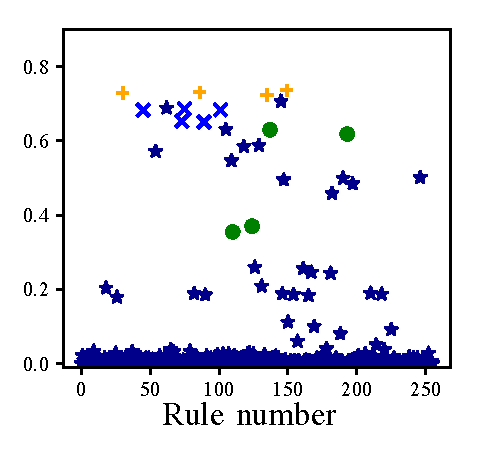
\includegraphics[width=\linewidth]{figures/nn}
    \caption{Neural network-based predictor}
      \label{subfig:nn_ent_one}
  \end{subfigure}

  \caption{Average cross entropy loss for the two predictor-based methods on all
    256 ECA. Rules are separated in several clusters. The
    count-based predictor (left plot) and neural network-based predictor (right
    plot) were applied with a neighborhood radius $r=1$ and $3$.}
\end{figure}

We note the similarity between this plot and the one from Figure
\ref{subfig:comp_scores}, with a roughly equivalent resulting classification of
ECA rules, with the exception of rules with low score. Rules that produce highly
disordered patterns are on top of the plot whereas the very simply behaving
rules are at the bottom. This indicates coherence between the two metrics.

\subsection{Neural network based predictor}

\begin{figure}[htbp]
  \centering
  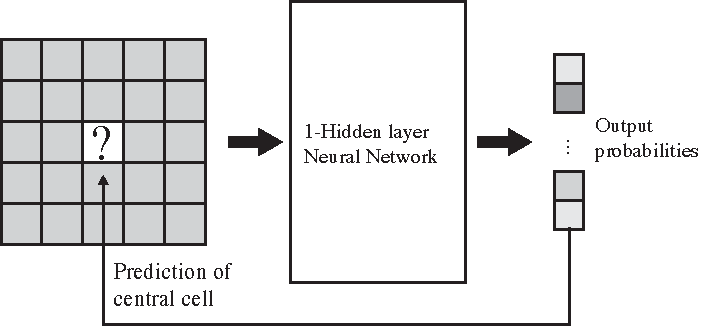
\includegraphics[width=.7\linewidth]{figures/nn_archi}
  \caption{Neural network architecture for predicting a central cell given its
    neighbors. Output probabilities are defined for all possible states of the
    central cell.}
  \label{fig:nn_archi}
\end{figure}

The frequency based predictor described above still has limitations:
\begin{itemize}
\item It does not take into account any redundancy in the input which may lead to
  suboptimal predictions (in a CA, very similar positions might have similar
  center cell state distribution, e.g. a glider in Game of Life should be
  recognized by the model no matter the rest of the neighborhood).
\item For the same reasons, when considering large window sizes, the number of
  possible neighborhood configuration gets much larger than the number of
  observed ones, leading to an input sparsity problem.
\end{itemize}
More sophisticated models can cope with above limitations by dealing with high
dimensional inputs without sparsity problems, and taking into account redundancy
of inputs and potential interactions between states for prediction.

We measure the cross-entropy loss of this simple model on the training set after
a standard learning procedure which is the same for all rules. The procedure is
applied to a one hidden layer neural network with a fixed hidden layer size. We
use a ReLU non-linearity for the hidden layer and a softmax to obtain the output
probabilities.

For $n$ possible states ${s_1, ..., s_n}$, a cell in state $s_k$ is represented
as a vector of 0s of size $n$ with a 1 in position $k$. The input to the network
is the concatenation of these cell vectors for all cells in the neighborhood.
The output of the network is a vector of size $n$ with the output probability
for each state.

Gradient updates are computed during training to minimize the cross-entropy loss
between outputs and target examples. For a timestep $T$, we use the training
procedure in order to minimize with respect to $\theta$ the following quantity,
\begin{align}
  L_\theta^{(T)} = - \frac{1}{N}\sum_{i=1}^N \sum_{k=1}^n
  \mathds{1}_{\{ s_k \}}\left(c_i^{(T)}\right)
  \log\left[f_\theta\left(n_{r,i}^{(T)}\right)_{s_k}\right]
  \label{eq:loss_network}
\end{align}
where the neural network depending on parameter $\theta$ is denoted $f_\theta$,
and $n_{r,i}^{(T)}$, the neighborhood of cell $i$ with radius $r$ at time $T$ is
defined in the same way as in eq.~\eqref{eq:loss_count}. Loss is computed with
respect to the testing set at time $T + \tau$ by computing the same quantity at
this subsequent timestep.

The training procedure is selected to achieve reasonable convergence of the loss
for the tested examples. It must be well defined and stay the same to allow for
comparison of the results across several rules. Score at timestep $T$ for a
delay $\tau$ is computed with the following formula
\begin{align}
  \mu_\tau = \dfrac{L^{(T)}}{L^{(T + \tau)}}
  \label{eq:main_metric}
\end{align}
where $L^{(T + \tau)}$ is the log probability of the automaton state at timestep
$T + \tau$ (defined in eq.~\eqref{eq:loss_network}) according to a model with
parameters learned during training at timestep $T$ and $L^{(T)}$ is the same as
in eq.~\eqref{eq:loss_network}. The value $\mu_\tau$ will be lower for easily
``learnable'' global states that do not translate well in future steps --- they
create more complexity or disorder --- thereby discarding slowly growing very
disordered structures. Higher values of $\mu_\tau$ correspond to automata that
have a disordered global state at time $T$ that can be transposed to future
timesteps relatively well. Those rules will tend to have interesting spatial
properties --- not trivially simple but not completely disordered because the
model transposes well --- as well as a large amount of overlap between a given
step and the future ones, indicating persistence of the spatial properties from
one state to another. We also selected the metric among other quantities
computed from $L^{(T)}$ and $L^{(T+\tau)}$ because it yielded the best score on
our experimental datasets.

\section{Experiments}\label{sec:experiments}

We carried out several experiments on a dataset of 500 randomly generated 3
states ($n=3$) rules with radius $r=1$. Those rules were manually annotated for
interestingness, defined as the presence of visually detectable non trivial
structures. The dataset contains 46 rules labeled as interesting and 454
uninteresting rules. Ranking those rules with the metrics introduced above
allows to study the influence of parameters and the adequacy between
interestingness as we understand it and what the metric measures.

The task of finding interesting rules can either be framed as a classification
problem or a ranking problem with respect to the score we compute on the
dataset. The performance of our metric can be measured with usual evaluation
metrics used on these problems, and notably the average precision (AP) of the
resulting classifier.

Average precision scores for the neural network and count-based methods for time
windows of 5, 50 and 300 timesteps are given in Table~\ref{experiments_table}.
Scores were computed on automata of size $256\times 256$ cells, ran for 1000
timesteps ($T + \tau = 1000$). Scores were computed for radii ranging from 1
cell (8 nearest neighbors) to 5 cells (120 neighbors), with a one layer neural
network containing 10 hidden units trained for 30 epochs with batches
of 8 examples. Best AP for each time window is shown in bold.
Results for the frequency lookup table predictor are only shown for $r=1, 2$
because of sparsity issues with the lookup table from $r=2$ and above making it
unpractical to use the table --- $3^{24}$ possible entries for the lookup table
with $r=2$ against only $256^2$ observed states.

\begin{table}[t!]
  \renewcommand{\arraystretch}{1}
  \caption{Experimental results - AP scores}
  \label{experiments_table}
  \centering
  \begin{tabular}{c|c|c|c|c|c}
    \toprule
    \bfseries Neural network& $r=1$ &  2  & 3  & 4 & 5\\
    \midrule
    5 steps & 0.387 & 0.448 & \bfseries 0.541 & 0.525 & 0.534\\
    50 steps & 0.377 & 0.433 & 0.517 & 0.491 & \bfseries 0.542\\
    300 steps &0.358 & 0.454 & 0.488 & \bfseries 0.527 & 0.525\\
    \midrule
    \bfseries Lookup table& $r=1$ &  2  & & &\\
    \midrule
    5 steps & 0.092 & 0.070&&&\\
    50 steps & 0.102 & 0.070&&&\\
    300 steps & 0.093 & 0.069&&&\\
    \bottomrule
  \end{tabular}

  \begin{flushleft}{This table shows the average precision (AP)
      scores obtained on the dataset of section \ref{sec:experiments} with the
      neural network-based and lookup table-based methods. Results are show for
      delays $\tau = 5, 50, 300$ and several radii values $r$.}\end{flushleft}
\end{table}

From these experiments, bigger radii appear to perform slightly better, although
not in a radical way. Since the number of neighbors scales with the square of
the radius, reasonably small radii might be a good trade-off between performance
and computational cost of the metric.

We also study the performance of our metrics --- lookup table and neural
network-based --- as inputs of a binary classifier against two simple baselines
on a random 70/30 split of our dataset. The first baseline classifies all
example as negative. The second baseline is based on compressed length as
defined in \parencite{zenilCompressionBasedInvestigationDynamical2010} and computed by choosing a pair
of thresholds that minimize mean square error when classifying examples in
between as positive --- this is based on the observation made in
Section~\ref{sec:compr-based-metr} that interesting rules have intermediate
compressed lengths. Results are in Table~\ref{experiments_table2} where only the
best radius is shown. The lookup table performs better than the baselines but
the neural network gives the best score.

\begin{table}[t!]
  \renewcommand{\arraystretch}{1.2}
  \centering
  \begin{tabular}{lm{.1\linewidth}m{.19\linewidth}m{.1\linewidth}m{.11\linewidth}}
    \toprule
    \bfseries  Metric & Baseline & Compressed length
    \parencite{zenilCompressionBasedInvestigationDynamical2010} &
    Lookup Table & Neural network \\ \midrule
    \bfseries Accuracy & 0.90 & 0.913 & 0.926 & \bfseries 0.953 \\ \bottomrule
  \end{tabular}
  \\[+8pt]
  \caption{Experimental results - Accuracy of each metric of complexity when
    used to classify which automatons do evolve interestingly, compared against
    the trivial all-negative baseline and the compressed length
    metric~\parencite{zenilCompressionBasedInvestigationDynamical2010}.}
  \label{experiments_table2}
\end{table}

Above experiments demonstrate the capability of our proposed metric to match a
subjective notion of interestingness of our labeling. For instance, the top 5
and top 10 scoring rules of the best performing configuration ($r=3$, $\tau =
5$) are all labeled as interesting, and top 100 scores contain 41 of the 46
rules labeled as interesting.

\section{Discussion}

In this section, we discuss the results obtained by using the metric of
\eqref{eq:main_metric} and the way they can be interpreted.

\paragraph{One dimensional cellular automata}
By applying the metric on the same example as before, we again obtain a
plot with a rule classification that matches a visual appreciation of
complexity of 1D CA. Results are shown on Figure~\ref{subfig:nn_ent_one}.
Similarly to the previous cases, rules we might label as interesting are
unlikely to be either at the top or bottom of the plot.

\paragraph{Two dimensional cellular automata}

Simulations conducted with 2D CA used grids of size 256$\times$256. Automata
were ran for 1000 steps (the metric is measured with respect to the reference
time $T = 1000$). Rules are defined with a table of transitions from all
possible neighborhood configurations with radius $r=1$ (3$\times$3 squares) to a
new state for the central cell. Unbiased sampling of rules, obtained by
uniformly sampling the resulting state for each transition independently,
overwhelmingly produces rules with a similar amount of transitions towards each
state and fails to produce rules without completely disordered behavior more
than 99\% of the time.

Therefore, we adopt a biased sampling strategy of the rules, selecting the
proportion of transitions towards each state uniformly on the simplex --- e.g
for 3 states we might get the triple $(0.1, 0.5, 0.4)$ and sample transitions
according to these proportions. This parametrization can be related to Langton's
lambda parameter \parencite{langtonComputationEdgeChaos1990} that takes into account the
proportion of transitions towards a transient (inactive) state and all the other
states. We obtain approximately 10\% interesting rules with this sampling as the
proportions of our experimental dataset show.

\begin{figure}[t]
  \centering
  \subfloat{
    \includegraphics[width=.38\linewidth]{figures/glid1}
  }\hfil
  \subfloat{
    \includegraphics[width=.38\linewidth]{figures/glid2}
  }
  \caption{Rules with 3 states that have spontaneously occurring glider
    structures. The gliders are the small structures that are outside of the
    center disordered zone. Some of them move along the diagonals while some
    others follow horizontal or vertical paths. Note that some repeating
    patterns occur also in the more disordered center zone.}
  \label{fig:gliders}
\end{figure}

\begin{figure}[t]
  \centering
  \subfloat{
    \includegraphics[width=.38\linewidth]{figures/2d_b_1}
  }\hfil
  \subfloat{
    \includegraphics[width=.38\linewidth]{figures/2d_b_2}
  }\hfil\setcounter{subfigure}{0} % Get the numbers right
  \subfloat[Timestep $T$]{
    \includegraphics[width=.38\linewidth]{figures/2d_c_1}
  }\hfil
  \subfloat[Timestep $T + 50$]{
    \includegraphics[width=.38\linewidth]{figures/2d_c_2}
  }
  \caption{Spontaneous glider formation and evolution is observed for some high
    scoring 2 states rules. Each row corresponds to a rule, with a 50 timesteps
    difference between the two columns. Gliders are marked with a gray square.
    Runs were initialized with a small 20 by 20 disordered square (uniformly
    sampled among possible configuration) in the center simulated for up to 400
    steps.}
  \label{fig:automat_glider}
\end{figure}

Using the neural network-based complexity metric, we were able to find rules
with interesting behavior among a very large set through random sampling. Some
of these rules are shown here. Figure~\ref{fig:automat_glider} displays three 2D
rules that were selected manually upon visual inspection among the 20 highest
scoring for metric $\mu_{50}$ (defined in eq.~\eqref{eq:main_metric}) of a sample
of 1700 randomly generated 2-states 3 by 3 neighborhood rules. For comparison,
Conway's Game of Life rule (GoL) ranks in the top 1\% of the 2500 rules
mentioned above for runs that do not end in a static global state. We observe
that spontaneous glider formation events appear to be captured by our metric.
Although gliders in cellular automata are a simple process that can manually be
created, detection of their spontaneous emergence within a random search setting
is a first step towards finding more complex macro structures that can emerge
out of simple components. Rules with low scores are overwhelmingly of the
disordered kind.

Figures~\ref{fig:gliders}, \ref{fig:micro} and \ref{fig:odd} show some three
states rules that were selected through random sampling on the simplex with the
neural-network based metric. They were selected among the 30 highest scoring
rules out of 2500 randomly selected 3 states rules. Their behaviors all involve
the growth and interaction of some small structures made of elementary cells.

All automata were initialized with a random disordered square of 20 by 20 cells
in the center. In the Figures mentioned above, colors were normalized with the
most common state set to blue. Figure~\ref{fig:gliders} shows rules that
spontaneously emit gliders that go through space in a direction until they
interact with some other active part of the automaton. Figure~\ref{fig:micro}
shows rules that generate small structures of between four and thirty cells that
are relatively stable and interact with each other. These elementary components
could be a basis for the spontaneous construction of more complex and bigger
components. Figure~\ref{fig:odd} shows some other rules from this set of high
ranking automata. They highlight the wide range of behaviors that can be
obtained with these systems. Interesting rules from our search process can be
found, along with other examples, in the form of animated
GIFs\footnote{\url{https://bit.ly/interesting_automata}}.

\begin{figure}[t]
  \centering
  \subfloat{
    \includegraphics[width=.38\linewidth]{figures/micro3}
  }
  \hfil
  \subfloat{
    \includegraphics[width=.38\linewidth]{figures/micro4}
  }
  \caption{Rules with 3 states that generate cell-like interacting structures.
    These patterns are either static or moving and can interact with one another
    to generate copies of themselves and other patterns. Note the very similar
    micro-structures that are repeated at several places in the space.}
  \label{fig:micro}
\end{figure}


\begin{figure}
  \centering
  \subfloat{
    \includegraphics[width=.38\linewidth]{figures/odd1}
  }
  \hfil
  \subfloat{
    \includegraphics[width=.38\linewidth]{figures/odd2}
  }
  \caption{Rules with surprising behaviors that are highly structured but
    complex. Those rules were selected among high-ranking rules for the
    neural-network based complexity metric. They all exhibit structurally non
    trivial behavior.}
  \label{fig:odd}
\end{figure}

For some of these rules interesting patterns appear less frequently in smaller
grids, indicating that the size of the space might impact the ability to
generate complex macro-structures. Increasing the size of the state space to
very large grids might therefore make it easier generating very complex patterns.

\section{Conclusion}\label{sec:conclusion}

In this chapter, we have proposed compression-inspired metrics for measuring a
form of complexity occurring in complex systems. We demonstrated its usefulness
for selecting CA rules that generate interesting emergent structures from very
large sets of possible rules. In higher dimensions where linear compression ---
as in gzip --- is not sufficient to find complex patterns, our metric is also
useful.

We study 2 and 3 states automata here and we plan to investigate the effects of
additional states or larger neighborhoods on the ability to evolve more
structures and obtain more interesting behaviors.

The dataset and code to reproduce our experiments and improvement on the results
reported are published on
GitHub\footnote{\url{https://github.com/hugcis/evolving-structures-in-complex-systems}}.
The metrics we introduce in this chapter could be used to design organized
systems of artificial developing organisms that grow in complexity through an
evolutionary mechanism. A possible path toward such systems could start by
creating an environment where computational resource allocation favors the
fraction of subsystems that perform the best according to our measure of
complexity.

The proposed metric is theoretically applicable to any complex system where a
notion of state of an elementary component and locality can be defined. With
these requirements fulfilled, we can build a similar prediction model that uses
information about local neighbors to predict the state of a component and
thereby assess the structural complexity of an input.

We believe that the capability of creating evolving systems out of such
elementary components and with few assumptions could be a step towards AGI. By
devising ways to guide this evolution in a direction we find useful, we would be
able to find efficient solution to hard problems while retaining adaptability of
the system. It might be suitable to avoid over-specialization that can happen in
systems designed to solve a particular task --- e.g. reinforcement learning
algorithms that can play games, and supervised learning --- by staying away from
any sort of objective function to optimize and by leaving room for open-ended
evolution.

\chapter{Visualization of computation in large-scale complex systems}
\label{cha:visu-comp-large}

  Emergent processes in complex systems such as cellular automata can perform
  computations of increasing complexity, and could possibly lead to artificial
  evolution. Such a feat would require scaling up current simulation sizes to
  allow for enough computational capacity. Understanding complex computations
  happening in cellular automata and other systems capable of emergence poses
  many challenges, especially in large-scale systems. We propose methods for
  coarse-graining cellular automata based on frequency analysis of cell states,
  clustering and autoencoders. These innovative techniques facilitate the
  discovery of large-scale structure formation and complexity analysis in those
  systems. They emphasize interesting behaviors in elementary cellular automata
  while filtering out background patterns. Moreover, our methods reduce large 2D
  automata to smaller sizes and enable identifying systems that behave
  interestingly at multiple scales.

\section{Introduction}
Cellular automata (CA) have been extensively studied since the 1960s. Originally
designed and studied to create artificial evolution from self-replication
\parencite{vonneumannTheorySelfreproducingAutomata1966,
  langtonSelfreproductionCellularAutomata1984}, previously studied cellular
automata simulations were often of relatively modest sizes. Only specific rules
with repetitive or predictable dynamics such as John Conway's Game of Life
\parencite{gardnerMathematicalGames1970} have been scaled up to larger grid sizes
($10^4 \times 10^4$ or more cells).

For complex phenomena such as artificial evolution to exist and be open-ended
within those simulated worlds, there needs to be sufficient ``capacity'' --- a
large enough state-space. In nature, complex and significantly different
dynamics often arise from uniform laws at a smaller
scale~\parencite{andersonMoreDifferent1972}. It seems unlikely that such complex
processes, like artificial evolution, could happen in too small CAs because
higher order dynamics do not have enough capacity to emerge. However, several
issues arise when scaling CAs to large sizes:

\begin{itemize}
\item Time complexity rapidly becomes a bottleneck. Updating a large number of
  cells is costly. Tricks such as caching of some of the computations can help,
  but do not always improve performance
  significantly~\parencite{gosperExploitingRegularitiesLarge1984}.

\item Memory complexity can also become an issue when dealing with numerous
  states, and especially grids in 3 dimensions and more. In that case, even the
  underlying rule of the system cannot be stored within reasonable memory
  capacity.

\item Visual inspection of these large grids is infeasible. Studying CA
  complexity is rendered difficult by the highly variable nature of emergent
  processes. It is especially the case for large-scale systems.

\end{itemize}
When working with such large systems, it is less relevant to focus on the local
behaviors at the single cell level. This is similar to other complex systems
like the weather, in which behaviors of individual atoms in a cloud are
irrelevant to large-scale air mass movements. Much richer behaviors can be
observed from studying large patterns' formation and their evolution. This
should also hold true for CAs; we further discuss this question in
\nameref{sec:conclusion-vc}.

\begin{figure}[th]
  \centering
  \includegraphics[width=.93\linewidth]{figures/rule18_small.pdf}
  \caption{\label{fig:rule18_small} \textbf{Hidden structures in rule 18 are
      uncovered by filtering the space-time diagram with our frequency
      histogram-based method}. \textbf{(a)} shows 300 timesteps of a randomly
    initialized rule 18 simulation. Notice the complex structures made visible
    in \textbf{(b)} with our method.}
\end{figure}

In this paper, we investigate techniques which can help us visualize large
space-time diagrams of CAs. We demonstrate that simple clustering and
coarse-graining techniques can be used in order to perceive structures which
cannot emerge on smaller grids. This is also useful for disordered cellular
automata with hidden structures as it is the case for the elementary cellular
automaton rule 18, illustrated in Figure~\ref{fig:rule18_small} --- more details
in~\nameref{sec:results}.

Reducing large grids to smaller sizes while preserving interesting behaviors
such as pattern formation is essential to apply to these CAs complexity metrics
designed to work on modestly sized
grids~\parencite{grassbergerQuantitativeTheorySelfgenerated1986,
  zenilCompressionBasedInvestigationDynamical2010,
  soler-toscanoCalculatingKolmogorovComplexity2014,
  zenilTwodimensionalKolmogorovComplexity2015}. Common metrics of complexity are
often limited by the number of components in the systems (number of cells in a
CA grid, timesteps, etc.) or may not be effective when small scale patterns are
less relevant than large-scale ones.

\section{Related work}

Previous work on coarse-graining cellular automata focused either on conserving
the main computational properties of CA rules through exact coarse-graining or
on filtering interesting behaviors without reducing the amount of computations.
Our work both highlights interesting behaviors and compresses the
representation, which we argue are necessary to study complexity in large
cellular automata.

\subsection{Coarse-graining in cellular automata}
Coarse-graining is an approximation procedure used to speed up computations in
systems made of many components. It originated
in~\parencite{levittComputerSimulationProtein1975} and is now widely used in physics
to model complex systems at various granularity levels, and is successful at
modeling bio-molecules \parencite{potoyanRecentSuccessesCoarsegrained2013,
  ingolfssonPowerCoarseGraining2014, kmiecikCoarseGrainedProteinModels2016}.

Exact coarse-graining of elementary cellular automata (ECA) has been
investigated extensively
in~\parencite{israeliComputationalIrreducibilityPredictability2004,
  israeliCoarsegrainingCellularAutomata2006}. Authors found ways of rewriting
one-dimensional CA rules into each other through coarse-graining of the
transition rule. They built a graph of equivalence of all 256 ECA and identified
some rules that do not admit any computational reduction. This indicates that
some cellular automata are accomplishing fundamentally more computations than
others.

\subsection{Filtering}

Filtering cellular automata (CA) was introduced to reduce a CA's behavior to its
most relevant parts. The goal is to extract relevant irregularities from a CA's
space-time diagram. Seminal work
by~\parencite{hansonAttractorbasinPortraitCellular1992,
  hansonComputationalMechanicsCellular1997} formalized the notion of domains and
coherent structures in cellular automata. They used a set of regular languages to
represent cellular automata dynamics and extract relevant behaviors such as
discontinuities between regular domains or ``particles''.
Figure~\ref{fig:rule110} shows a filtering example for cellular automaton rule
110 --- in Wolfram's numbering.

A filtering method similar to our proposed frequency-based coarse-graining ---
originally presented as a complexity metric for cellular automata --- is
introduced in~\parencite{wuenscheClassifyingCellularAutomata1999}. The author
proposes to progressively filter out cells in cellular automata's space-time
diagrams according to read frequency of the rule table. Cells that originated
from frequent rule table lookups are set to a quiescent or null state. The
choice of threshold has to be decided by a user for each rule. Another notable
difference is the method aims at making visualization of gliders easier without
reducing the size of the grid or making more compact representations.

More recent work by~\parencite{shaliziAutomaticFiltersDetection2006} uses the
combination of a modified Lyapunov exponent approach with \emph{statistical
  complexity} \parencite{shaliziQuantifyingSelfOrganizationOptimal2004} to underline
complex behaviors. However, the first method requires repeated perturbations and
simulations of the system to study its sensitivity.

\subsection{Scaling-up cellular automata}
Hashlife \parencite{gosperExploitingRegularitiesLarge1984} and other Game of
Life-specific optimizations enable simulating a large number of cells for
numerous timesteps. Nonetheless, these algorithms essentially exploit input
redundancy. The regularity in patterns allowing such optimizations might
indicate a lack of novel patterns being generated by the system.

This also means that Game of Life-based simulations are computationally
reducible to a much simpler system, indicating that its computations are
inefficient~\parencite{wolframNewKindScience2002}. An optimally complex-behaving
computational model should be impossible to predict except when computing its
actual evolution step by step.

In the following, we used coarse-graining as a method for scaling down CAs in
both time and space in order to make visualization of larger patterns and
complex behaviors easier. The underlying fine-scale computations may be
essential for these larger patterns to appear, hence the necessity to keep them.
However, analogous to many natural processes (swarms, chemistry, cells in an
organism, DNA), interesting behaviors might not be observable at the level of
individual components --- or small groups of components (individuals, single
cells or molecules in the examples above). We view coarse-graining as a way to
reduce a cellular automaton's space-time diagram to its most relevant parts
while keeping primary dynamics in the background. The resulting diagram would
ideally be an irreducible system.

\section{Proposed coarse-graining of cellular automata}
For reasons stated above, we introduce coarse-graining methods for cellular
automata that are not reversible --- information is discarded in the process.
This process does not attempt to find shortcuts for the computations of a
cellular automaton, but rather to selects relevant parts of the space-time
diagram and discards information irrelevant to the core behavior. For example, a
standard glider in Game of Life spanning $3\times 3$ cells could be replaced
with a single cell moving diagonally when coarse-graining by a factor 3. This is
because the actual oscillator's dynamics might not be relevant at this coarser
scale.

Coarse-graining is akin to constructing \emph{supercells} from blocks of individual
cells. These supercells are assigned a new state and form a coarser partitioning
of the initial grid which can be studied as its own system. In particular,
complexity metrics or further coarse-graining can be applied to this new grid.

\subsection{Frequency histogram coarse-graining}\label{sec:simple-hier-coarse}

A simple coarse-graining is achieved by mapping blocks to a single
\emph{supercell} state according to the probability of this configuration
appearing, given a previously constructed model. The easiest way to think of it
is with a simple frequency counting model of the distribution of $2\times 2$
blocks in a 2D CA\@. For a 2-state automaton, there are 16 possible supercell
configurations. The simplest model for the occurrence of these blocks is their
empirical frequency. Let us consider a CA with $N$ blocks of $2\times 2$ cells,
let $S^{(in)} = \{\mathtt{0000}, \mathtt{0001}, \mathtt{0010}, \ldots,
\mathtt{1111}\}$ be the set of $2\times 2$ blocks and $s_i \in S^{(in)}$ be a
given supercell. The probability $p_i$ of observing supercell $i$ on a grid $G$
is estimated with
\begin{equation}
  p_i = \dfrac{\text{count}_G(s_i)}{\sum_{j\in S^{(in)}}\text{count}_G(s_j)}
  \label{eq:stat_est}
\end{equation}
where $\text{count}_G(s_i)$ is the number of blocks matching $(s_i)$ in $G$.

Supercells can then be assigned a particular state. We call the corresponding
mapping $f: S^{(in)} \mapsto S^{(out)}$. $S^{(out)}$ can be chosen depending on
the desired output or use. For instance, with $S^{(out)} = \{0, 1\}$ we can
define $f$ to map each supercell $s_i$ as follows:
\begin{align}
  f(i) = \begin{cases}
    \mathtt{0} &\quad\text{if }\ p_i\geq \alpha\\
    \mathtt{1} &\quad\text{if }\ p_i< \alpha
  \end{cases}
        \label{eq:alpha}
\end{align}
where $\alpha$ is a chosen threshold.

\subsubsection{Partitioning the histogram.}
This method can be understood as partitioning the histogram of supercell
frequency. In equation~\eqref{eq:alpha}, supercells with low probability
--- with higher self-information --- are mapped to state \texttt{1} whereas
commonly occurring states are mapped to \texttt{0}.

Choosing a partition of the histogram is equivalent to selecting a suitable
$\alpha$ --- scalar for two output states, or vector $\mathbf{\alpha} =
(\alpha_1, \ldots, \alpha_n)$ for $n$ output states. Therefore, one can map
supercells to any number of target states (three or more) by partitioning the
frequency histogram into any number of bins. Supercell distribution can be
anything between uniform and very unbalanced, with a few supercells being
overwhelmingly represented (background) and only a few occurrences of other
configurations. The chosen partitioning has to deal with both situations equally
well. In the following, we use a uniform partitioning of the area under the
negative log-histogram for elementary cellular automata --- supercells are
divided into two bins of equal summed negative logarithmic probability. For 2D
CAs, we use the same method but with quadratic partition of the histogram
($1/k^2$ instead of $1/k$, with $k$ the number of output states, chosen because
of better visual results).

\subsubsection{Dithering.}\label{sec:dithering}
Histogram partitioning introduces another set of parameters to be manually
tuned, adding complexity to the procedure. An alternative way to produce an
output image from the histogram is to use dithering. Dithering is an image
processing technique commonly used to reduce large visual artifacts induced by
quantization errors. Noise is added to the image during the quantization process
to make the average local value of a set of pixels as close to their target
continuous value as possible. The resulting image is created so as to match
target continuous values with discrete values only --- cell states in the grid.
It can be seen as another way of partitioning the histogram with variable
thresholds that depend on a running quantization error.
Figure~\ref{fig:close-up} shows a comparison of dithering and regular histogram
partitioning (Floyd–Steinberg's algorithm was used
\parencite{floydAdaptiveAlgorithmSpatial1976}).

\setlength{\fboxsep}{0pt}
\begin{figure}[th]
  \centering
  \begin{subfigure}{.32\linewidth}
    \fbox{\centering
    \includegraphics[width=\linewidth]{figures/step_large.png}}
    \caption{\label{subfig:normal}Original CA}
  \end{subfigure}
  \hfill
  \begin{subfigure}{.32\linewidth}
    \fbox{\centering
    \includegraphics[width=\linewidth]{figures/freq_cg_large.png}}
    \caption{\label{subfig:no-dithering}w/out dithering}
  \end{subfigure}
  \hfill
  \begin{subfigure}{.32\linewidth}
    \fbox{\centering
    \includegraphics[width=\linewidth]{figures/dither_cg_large.png}}
    \caption{\label{subfig:dithering}with dithering}
  \end{subfigure}

  \caption{\label{fig:close-up}\textbf{Close-up view of coarse-graining effects
      on a 4-states CA rule} (1 shade of blue per state). Both coarse-graining
    methods conserve many of the interesting structures. Dithering introduces
    additional artifacts on regular backgrounds. Fig.~\ref{subfig:normal} shows
    actual states in the CA simulation on a $128 \times 128$ grid.
    Fig.~\ref{subfig:no-dithering} is a coarse-grained version
    of~\ref{subfig:normal} with histogram coarse-graining, the grid is $64
    \times 64$ cells.\ref{subfig:dithering} is obtained with histogram
    coarse-graining and dithering (see \nameref{sec:dithering}).}
\end{figure}


\subsubsection{Visualization.}
One advantage of this frequency histogram-based method is that it naturally
highlights rarer events in the simulation grid, creating a ``heatmap'' of the
simulation's activity. Since we sort supercells according to their observed
frequency, the right choice of colors --- e.g.\ progressively darker gradient
--- can lead to automatic highlighting of active regions of a cellular
automaton. Figure~\ref{fig:gol_comparison} shows the same simulation both
unprocessed and downscaled by a factor of 4 with coarse-graining. Although much
coarser, Figure~\ref{subfig:gol_cg} is more readable than the base version,
which is helpful when dealing with large grids\footnote{Several figures in this
  paper have animated versions, accessible at the paper's project page
  \projecturl}.

\begin{figure}[th]
  \centering
  \begin{subfigure}{.48\linewidth}
    \fbox{
    \centering
    \includegraphics[width=\linewidth]{figures/viz10460682591249143347/base-76.png}}
    \caption{\label{subfig:gol}Base grid}
  \end{subfigure}
  \hfill
  \begin{subfigure}{.48\linewidth}
    \fbox{
    \centering
    \includegraphics[width=\linewidth]{figures/viz10460682591249143347/coarse-76.png}}
    \caption{\label{subfig:gol_cg}Coarse-grained}
  \end{subfigure}

  \caption{\label{fig:gol_comparison}\textbf{Side-to-side comparison of a CA
      simulation and its coarse-grained version}. The first simulation is $256
    \times 256$ cells and the second has been coarse-grained to $64\times 64$.
    Notice the interesting patterns on Figure~\ref{subfig:gol} are hardly
    distinguishable. They are highlighted by histogram-based coarse-graining in
    Figure~\ref{subfig:gol_cg}.}
\end{figure}


\subsubsection{Hierarchical coarse-graining.}
The above procedure can be applied recursively to the same cellular automaton or
with larger block sizes to get a progressively coarser representation. Since
information is systematically discarded in the process, it cannot be applied any
number of times. For this reason, many 2D CAs exhibiting interesting behaviors at
the micro-level but not at the macro-level have no remaining visible structure
after reducing their scale several times with this method.

Because a simple model like frequency counting can be estimated quickly,
hierarchical coarse-graining is easily applied to large grids, reducing the size
by a factor of $n$ (block size) every time. For instance, this property makes it
suitable to search the cellular automata rule space for CAs behaving
interestingly at multiple coarse-graining levels simultaneously.

\subsection{Clustering}

Another way to convert blocks of cells for coarse-graining is to distribute
these blocks into a small number of clusters, where each group becomes the new
coarse state.

Several distance functions may apply here, the most natural of which being
Hamming distance, which measures how many states differ between two
positions~\parencite{hammingErrorDetectingError1950}. It is defined for two strings
of equal length $n$, $s_1 = [s_{(1, 1)}, \ldots, s_{(1,n)}]$ and $s_2 =
[s_{(2,1)}, \ldots, s_{(2,n)}]$, as the number of positions where the two
strings differ:
\begin{align}
  \sum_{k = 1}^n \mathds{1}\left\{\ s_1^{(k)}  \neq s_2^{(k)}\right\}.
\end{align}

A supercell of $N\times N$ cells of a CA can be converted into a string to be
compared to other blocks with the Hamming distance. For CAs, we limit ourselves
to strings of digits representing states, i.e. $s_{(i,j)} \in \mathbb{N}$. We
use a vanilla implementation of the K-means algorithm where clusters' centers
are computed using a continuous average of position vectors rounded to nearest
integer values. Clusters are initialized with randomly selected observations.

\subsection{Autoencoders for coarse-graining}

Instead of just relying on the amount of information of a given supercell's
configuration, one can also try to automatically find a relevant representation
with dimensionality reduction methods. Autoencoders are neural networks composed
of an encoder part and a decoder part, originally designed to identify principal
components of a collection of data
points~\parencite{baldiNeuralNetworksPrincipal1989,
  hintonConnectionistLearningProcedures1989,
  kramerNonlinearPrincipalComponent1991}. An encoder neural network converts
data to a \emph{latent} vector of smaller dimension than the original input.
Then, a decoder neural network reconstructs a vector with the same dimension as
the input from this encoded \emph{latent} representation.These models can
automatically find an optimal constrained representation through minimizing a
reconstruction loss between the original input and the reconstructed output.

We denote the encoder network with $E$ and the decoder network with $D$. We frame
the reconstruction problem as a $N$ class classification problem with multiple
components --- one class per input state, one component for each cell of the $K$
cells in a block. The reconstruction loss is the component-wise cross-entropy
between the state of each input cell and the reconstructed state after $D \circ
E$ is applied.

\begin{figure}[th]
  \centering
  \includegraphics[width=\linewidth]{figures/autoencoder.pdf}
  \caption{\label{fig:autoencoder} \textbf{Diagram of the autoencoder
      architecture used for coarse-graining}. A block of $6\times 6$ cells is
    encoded in a vector of fixed dimension. There are 3 components in the
    example. They can either represent a RGB color or a 3 states smaller
    automaton.}
\end{figure}

Figure~\ref{fig:autoencoder} illustrates the autoencoder layout for
coarse-graining. By adjusting the block size and dimension of the encoded
vector, one can influence the amount of information conserved during encoding.
Naturally, smaller blocks will be more easily represented in lower dimension.

The encoder has a softmax layer to ensure the coded state's components sum to
one. Therefore, one can view this coded supercell as a mixture of states which
can either be kept as is or converted to a discrete state by keeping the maximal
component only. They are trained with stochastic gradient descent until
convergence.

\section{\label{sec:results}Results}

We evaluate our proposed coarse-graining methods in the following two different ways:
\begin{itemize}
\item We compare our results on elementary cellular automata (ECA) to previous
  works on particle and domain filtering.
\item We use a metric which evaluates complexity of CAs introduced
  in~\parencite{cisnerosEvolvingStructuresComplex2019} in order to compare our
  methods' complexity metric scores of the coarse-grained systems and contrast
  the scores against a standard image processing baseline that computes local
  average of neighbouring cells followed by downscaling the grid. Using the
  complexity metric we measure to what extent the interesting behavior of
  cellular automata is conserved after coarse-graining compared to this image
  processing baseline.
\end{itemize}

In the following we begin by showing that a simple histogram-based
coarse-graining is effective at detecting structures (such as gliders) in ECA
space-time diagrams. Our method achieves results comparable with previous work,
while being simpler to apply.

\subsection{Domains and filtering}

In the space-time diagrams of cellular automata, moving structures such as
gliders are embedded in uniform or periodic backgrounds, or ``domains''. This
domain is different depending on the rule: some ECAs have uniform backgrounds,
checkerboard backgrounds or more complicated patterns (e.g.\ rule
110).~\parencite{crutchfieldTurbulentPatternBases1993} also identified chaotic
domains, which cannot support regular gliders but have ``walls'' and
``particles''. Those correspond, respectively, to boundaries between two chaotic
domains and propagating defects (localized structures with a pattern different
from the domain) within a domain.

Our proposed coarse-graining methods offer interesting perspectives to filter
cellular automata's space-time diagrams, which enables identifying gliders and
studying the formation of large-scale patterns. We find that a simple histogram
coarse-graining achieves results comparable to those reported
in~\parencite{hansonAttractorbasinPortraitCellular1992,
  elorantaKinkCellularAutomaton1992, hansonComputationalMechanicsCellular1997,
  wuenscheExploringDiscreteDynamics2011} for ECA rules 18 and 54. A similar
approach was undertaken in \parencite{wuenscheClassifyingCellularAutomata1999} in
which the authors used the entropy of rule table lookup frequencies to filter
out regular domains in the space-time diagrams of cellular automata and to
identify gliders and domain boundaries. However, Wuensche's approach described
in~\parencite{wuenscheClassifyingCellularAutomata1999} does not attempt to downscale
space-time diagrams.

\subsection{Results on elementary cellular automata}

\begin{figure}[th]
  \centering
  \includegraphics[width=\linewidth]{figures/rule18.pdf}
  \caption{\label{fig:rule18} \textbf{Space-time diagrams for rule 18 in
      elementary cellular automata.} \textbf{(a)} Standard rule 18 space-time
    diagram, starting from a random position. \textbf{(b)} Filtered domain with
    our frequency coarse-graining (even). \textbf{(c)} Our domain boundaries
    extracted from the filtered domains in \textbf{(b)}. \textbf{(d)} Domain
    boundaries computed according to
    \parencite{hansonAttractorbasinPortraitCellular1992}. Note that \textbf{(a)}
    shows semi-chaotic behaviour, which is hard to interpret, whereas our method
    \textbf{(b)} highlights distinct domains within the disordered space-diagram
    in (a). The detected domains and domain boundaries from previous work (d)
    and ours (c) are very similar.}
\end{figure}

We apply frequency histogram-based coarse-graining on elementary cellular
automata (ECA) and obtain space-time diagrams with suppressed background
domains. Resulting partitions of ECAs' space-time diagram are similar to results
reported by~\parencite{hansonAttractorbasinPortraitCellular1992,
  hansonComputationalMechanicsCellular1997}. Figure~\ref{fig:rule18}\textbf{(a)}
and~\ref{fig:rule54}\textbf{(a)} show the space-time diagrams of rules 18 and 54
with random initialization. Boundaries between different background patterns in
both Figures were obtained with coarse-graining; they are similar to boundaries
obtained by Hanson and Crutchfield. We also observe the propagation of many of
the same particles and defects without any prior information about the cellular
automaton rule.

Particles in Rule 54 have been used to implement
computations~\parencite{boccaraParticlelikeStructuresTheir1991,
  pivatoSpectralDomainBoundaries2007,
  martinezCompleteCharacterizationStructure2014}. Because the presented
reduction reduces the size of the grid, it can merge some of those particles,
sometimes resulting in ambiguities and gaps. However, our goal here is not to
precisely describe particle interactions in order to manipulate or construct
complex computations manually. Underlying computations described in the works
above are still happening within our reduced CA simulation. We consider the
\emph{apparent} destruction of some of these fine-scale details acceptable in
order to discover larger-scale complex behavior.

Our method is also arguably much simpler than computational mechanics (used by
Hanson and Crutchfield) which requires some reverse-engineering of the rule and
the construction of a finite-state transducer to generate output symbols.
Although full automation has been demonstrated, this method introduces
significant overhead~\parencite{rupeLocalCausalStates2018}. On the other hand, our
method is sensitive to the quality of statistical estimation of the frequency
histogram (see equation~\eqref{eq:stat_est}) and needs enough input examples to
achieve a reasonable result --- examples in Figure~\ref{fig:rule18}
and~\ref{fig:rule54} used simulations with the width of 3000 cells, ran for 6000
timesteps to obtain reliable pattern frequency estimates.

In the Figures, we used the coarse-graining method introduced
in~\nameref{sec:simple-hier-coarse}. Space-time diagrams are coarse-grained by a
factor 2 to a binary automaton --- each cell corresponds to a 2-cell block.
These binary coarse-graining results in the Figures are labeled \textbf{(c)}.
Because of the statistical nature of the domains of these 1D ECA's and the use of
blocks of size 2, filtered domains differ depending on the starting position of
coarse-graining. We distinguish an odd and even filtered domain.

Figure~\ref{fig:rule18}\textbf{(c)} is obtained by applying the element-wise
\texttt{OR} operator to both the even and odd domain diagrams to merge them into
a single space-time diagram. Figure~\ref{fig:rule54}\textbf{(c)} is obtained by
computing differences between neighboring cells after the filtering process to
highlight lines. Figure~\ref{fig:rule110} is another example showing filtering
of particles in rule 110.


\begin{figure}[th]
  \centering
  \includegraphics[width=\linewidth]{figures/rule54.pdf}
  \caption{\label{fig:rule54} \textbf{Space-time diagrams for rule 54}.
    \textbf{(a)} Space-time diagram of standard rule 54, starting from a random
    position. \textbf{(b)} Filtered domain with our frequency coarse-graining
    (even). \textbf{(c)} Particles filtered from the domains in \textbf{(b)
      using our method}. \textbf{(d)} Domain boundaries computed using
    computational mechanics \parencite{hansonComputationalMechanicsCellular1997}.
    Please note that particles are detected equally well using computational
    mechanics (d) and our (simpler) frequency-based method (c). Some close-by
    particle trails are merged using our method.}
\end{figure}

\begin{figure}[t]
  \centering
  \includegraphics[width=\linewidth]{figures/rule110.pdf}
  \caption{\label{fig:rule110} \textbf{Spate-time diagram of rule 110 (\textbf{a})
      and filtered particles using our histogram-based coarse-graining
      (\textbf{b})}. Structures propagating in time (vertical axis) and space
    (horizontal axis) become clearly visible in \textbf{(b)} as vertical and
    diagonal lines.
    %\textbf{(b)} shows the same structures with the regular
    %background domain filtered out with our method.
    }
\end{figure}
\subsection{Complexity metrics and coarse-graining}

\setlength{\fboxsep}{0pt}
\begin{figure}[th]
  \centering
  \begin{subfigure}{.48\linewidth}
    \fbox{\centering
      \includegraphics[width=\linewidth]{figures/13220943837485080965/19_rule_downscale_13220943837485080965-20.png}}
    \caption{\label{subfig:downscale3} Downscaling by averaging}
  \end{subfigure}
  \begin{subfigure}{.48\linewidth}
    \fbox{\centering
      \includegraphics[width=\linewidth]{figures/13220943837485080965/19rule_coarsed_13220943837485080965-20.png}}
    \caption{\label{subfig:histogram3} Histogram}
  \end{subfigure}
  \begin{subfigure}{.48\linewidth}
    \fbox{\centering
      \includegraphics[width=\linewidth]{figures/13220943837485080965/19rule_kmeans_13220943837485080965-20.png}}
    \caption{\label{subfig:kmeans3} K-means}
  \end{subfigure}
  \begin{subfigure}{.48\linewidth}
    \fbox{\centering
    \includegraphics[width=\linewidth]
    {figures/13220943837485080965/19rule_autoencoder_13220943837485080965-20.png}}
    \caption{\label{subfig:autoencoder3}Autoencoder}
  \end{subfigure}
  \caption{\label{fig:qualitative}\textbf{Qualitative comparison of
      coarse-graining methods}. Simulations are on grids of $4096 \times 4096$
    cells coarse-grained to $512 \times 512$. Lines are barely visible with
    downscaling~\ref{subfig:downscale3}, but are visible
    in~\ref{subfig:histogram3}-\ref{subfig:autoencoder3}. Coarse-graining helps
    visualize linear structures that would be hard to see otherwise.}
\end{figure}

Coarse-graining is not only useful for detecting gliders and domains in
space-time diagrams, but also as a tool to visualize large CAs. To evaluate the
quality of our proposed coarse-graining methods, we compare complexity scores
computed according to~\parencite{cisnerosEvolvingStructuresComplex2019} for different
coarse-graining methods. This metric was shown to correlate well with a user
study of interesting automata. It uses neural networks to estimate how easy it
is to learn a compressed representation of a CA\@. We also computed the scores on
downscaled CAs as a baseline. Local averaging is used for downscaling, with each
block of $N$ cells being replaced by its average value rounded to the nearest
integer state.

Experiments begin by sampling 3600 cellular automata rules with 3 or 4 states.
We apply the complexity metric on a randomly initialized simulation on a $512
\times 512$ grid of cells. The top 100 rules with the highest complexity scores,
which should correspond to rules with interesting behaviors, are then used for
coarse-graining. We apply coarse-graining on grids of $4096 \times 4096$ cells,
scaling the grid down by a factor of $8$, and compute the complexity metric also
on the reduced grid. Figures reported in Table~\ref{experiments_table-vc} are
percentages of rules still considered interesting (above the selection threshold
for the first step of the process) after coarse-graining. The higher this number
is, the more a method is able to conserve complex and interesting behaviors
after the reduction.

\begin{table}[t!]
  \centering
  \begin{tabular}{ccccc}
    \toprule
       Local-averaging & K-Means & Histogram & Autoencoder\\
     baseline &  & & \\
    \midrule
      19.3\%  & 40.4\% & 82.4\% & 84.2\%\\
    \bottomrule
  \end{tabular}
  \label{experiments_table-vc}
  \caption{\textbf{Experimental results --- Percentage
      of rules classified as interesting after reduction with our 3 proposed
      methods (K-means, Histogram, Autoencoder), compared to a local averaging baseline.}}
\end{table}

Results in Table~\ref{experiments_table-vc} suggest that using our proposed methods
seems largely beneficial for studying complexity in large systems.
% when usual metrics become impractical.
Histogram and autoencoder methods are superior to downscaling using k-means and
local averaging. This could be attributed to the fact that contrary to the
latter two, the histogram and autoencoder both represent well anomalies (rare
events). This is because rare events are explicitly captured and kept by the
histogram method. They also represent useful information that may be kept for
the reconstruction using the autoencoder.

\subsection{Discussion}\label{sec:discussion}

Downscaling by local averaging is not an effective solution to the
coarse-graining problem for several reasons. In particular, it tends to favor
the majority state in a supercell because of the averaging effect. Thin
structures spanning only few cells placed on a uniform background are likely to
disappear after coarse-graining although they may still be relevant with respect
to the large-scale patterns. The histogram-based method explicitly encodes those
more rare events in a supercell, even if their size is relatively small compared
to the supercell size.
%The autoencoder may automatically encode this
%information too because those few cells are more useful to reconstruct the
%initial supercell than the background.

Figure~\ref{fig:qualitative} is a qualitative comparison of coarse-graining
methods. This cellular automaton was selected from the experimental dataset.
When simulated on large grids, it generates large linear structures that are
4-cells wide. These structure disappear after downscaling by averaging because
the background dominates the average. Other methods correctly highlight these
structures when downscaling the grids by a factor of 8. In
Figure~\ref{fig:dynamics_levels}, we show another rule that was selected for its
high complexity score at multiple coarse-graining scales from our dataset. The
CA has significantly different dynamics depending on the chosen scale.
Example~\ref{subfig:single} is a spontaneously occurring stable oscillating
glider with period 3. Large structures emerge from these simple gliders when
observing large grids. The online project page\footnote{\projecturl} shows
animated example for Figure~\ref{fig:dynamics_levels}, emphasizing the advantage
of using coarse-graining for visualization.

A crucial advantage of the frequency histogram method is its speed and ease of
implementation compared to autoencoders. Other than a few hyper-parameters for
partitioning the histogram, no training or tuning is needed to produce the
coarse-grained output.

\begin{figure}[ht]
  \centering
  \begin{subfigure}{.052\linewidth}
    \fbox{\centering
    \includegraphics[width=\linewidth]{figures/viz5413567812493154659/single_glider.png}}
    \caption{\label{subfig:single}}
  \end{subfigure}
  \begin{subfigure}{.45\linewidth}
    \fbox{\centering
    \includegraphics[width=\linewidth]{figures/viz5413567812493154659/mult_glider.png}}
    \caption{\label{subfig:mult_glider} $128 \times 128$ cells}
  \end{subfigure}
  \begin{subfigure}{.45\linewidth}
    \fbox{\centering
    \includegraphics[width=\linewidth]{figures/viz5413567812493154659/mult_glider_larger.png}}
  \caption{\label{subfig:mult_glider_larger} $512 \times 512$ cells}
  \end{subfigure}
  \begin{subfigure}{.48\linewidth}
    \fbox{\centering
      \includegraphics[width=\linewidth]{figures/viz5413567812493154659/waves_b.png}}
    \caption{\label{subfig:waves_b} $2048 \times 2048$ cells coarse-grained to $256 \times 256$.}
  \end{subfigure}
  \hfill
  \begin{subfigure}{.48\linewidth}
    \fbox{\centering
      \includegraphics[width=\linewidth]{figures/viz5413567812493154659/waves_c.png}}
    \caption{\label{subfig:waves_c} $4096 \times 4096$ cells coarse-grained to $256 \times 256$.}
  \end{subfigure}
  \caption{\label{fig:dynamics_levels} \textbf{Changing CA dynamics at multiple
      scales}. (a) shows a single glider, oscillating between 3 positions. Such
    gliders emerge spontaneously from a random initialization of a small grid as
    shown in (b). When scaling the grid up, trails of gliders begin to appear,
    creating moving straight and diagonal lines as shown in (c). Scaling-up even
    more, individual gliders are not visible anymore, as shown in (d). In an
    even larger grid, shown in (e), many more triangular-shaped waves travel and
    collide with each other. Please note that (d) and (e) are coarse-grained to
    $256 \times 256$, otherwise the patterns are not visible.}
\end{figure}


% \begin{figure}[th]
% \begin{subfigure}{.48\linewidth}
%   \centering
%   \includegraphics[width=\linewidth]
%   {figures/3904718678772130032_autoencoder/3904718678772130032_autoencoder-20.png}
%   \caption{\label{fig:autoencoder1}Autoencoder}
% \end{subfigure}
% \begin{subfigure}{.48\linewidth}
%   \centering
%   \includegraphics[width=\linewidth]{figures/3904718678772130032_coarsed/3904718678772130032_coarsed-20.png}
%   \caption{\label{fig:histogram1}Histogram}
% \end{subfigure}
% \end{figure}

% \begin{figure}[th]
%   \begin{subfigure}{.48\linewidth}
%     \centering
%     \includegraphics[width=\linewidth]
%     {figures/18072167875025464602_autoencoder/18072167875025464602_autoencoder-20.png}
%     \caption{\label{fig:autoencoder2}Autoencoder}
%   \end{subfigure}
%   \begin{subfigure}{.48\linewidth}
%     \centering
%     \includegraphics[width=\linewidth]
%     {figures/18072167875025464602_coarsed/18072167875025464602_coarsed-20.png}
%     \caption{\label{fig:histogram2} Histogram}
%   \end{subfigure}
% \end{figure}

\section{Conclusion\label{sec:conclusion-vc}}

We intend to use these coarse-graining methods to find cellular automata (CA) which
exhibit interesting behaviors at multiple scales.
Figure~\ref{fig:dynamics_levels} shows an example of such a CA\@. We observe
various dynamics depending on the scale, from simple oscillating gliders to
large wave-like patterns composed of thousands of gliders. It demonstrates that
observing multi-scale behaviors within those automata is possible. The existence
of 2D cellular automata with disordered behaviors at the smallest level but
organized at coarser scales, similar to hidden patterns in rule 18, would also
be of great interest.

Cellular automata are powerful computational models. Some of them have been
shown to be Turing-complete, and can thus be expected to support arbitrarily
complex computations~\parencite{berlekampWinningWaysYour2001,
  cookUniversalityElementaryCellular2004}. Naturally, most interesting CAs
spontaneously generate a fraction of available computations at a time, usually
supporting a few stable oscillators or moving structures. Proofs of universality
for these CAs required careful design of computational devices out of these
stable oscillators and structures, resulting in very brittle and inefficient
universal computers. In practise, only elementary functions --- such as density
classification, binary addition, etc. --- can be implemented. This requires
searching for CA rules specifically targeted at a particular
function~\parencite{mitchellEvolvingCellularAutomata1996, wolframNewKindScience2002,
  sapinResearchCellularAutomaton2003}. Hierarchies are central to naturally
occurring complex phenomena~\parencite{simonArchitectureComplexity1962}, and may be
required for robust and complex processes to emerge in CAs.

Viewing space-time diagrams of cellular automata is akin to visualizing a
foreign computer design. Cellular automata are manipulating information,
registers and instructions in parallel in the form of cell states. We believe
visualization tools proposed in this paper can help understand computations in
those unconventional computers. By reducing available information to its
essential parts, we attempt to distill the content of the space-time diagram
with as little prior information as possible. Future work could focus on
identifying some known simple computational primitives within cellular automata
and understanding how our visualization can help to find them.

These methods also enable apprehending large grid sizes for which even image
processing algorithms begin to show limitations. Complexity metrics and CA
classification techniques can be extended to these reduced large grids and could
lead to the discovery of CAs with --- similar to life and physical processes ---
significantly different dynamics at multiple scales that could in turn be a
basis for artificial evolution.

\chapter{Learning efficiency in deep reservoir computing}
\label{cha:learn-effic-compl}

It is common to evaluate the performance of a machine learning model by
measuring its predictive power on a test dataset. This approach favors
complicated models that can smoothly fit complex functions and generalize well
from training data points. Although essential components of intelligence, speed, 
and data efficiency of this learning process are rarely reported or compared
between different candidate models. In this chapter, we introduce a benchmark 
of increasingly difficult tasks together with a data efficiency metric to measure 
how quickly machine learning models learn from training data. We also highlight 
that within complex systems, there are computations taking place that can be 
harnessed for various purposes. To that end, we compare the learning speed of 
some established sequential supervised models, such as RNNs, LSTMs, or Transformers, 
with relatively less-known alternative models based on reservoir computing, which 
is a tool for harvesting the computations happening within a complex system.
 The proposed tasks require a wide range of computational
primitives, such as memory or the ability to compute Boolean functions, to be
effectively solved. Surprisingly, we observe that reservoir computing systems
that rely on dynamically evolving feature maps learn faster than fully
supervised methods trained with stochastic gradient optimization while achieving
comparable accuracy scores. The code, benchmark, trained models, and results to
reproduce our experiments described in this chapter are available at
{\small\url{https://github.com/hugcis/benchmark_learning_efficiency/}}.


\section{Introduction}
Most machine learning models are evaluated by measuring performance on a
specific dataset or task. Learning efficiency -- the ability to learn,
generalize, and adapt quickly from a few examples -- is crucial for practical
intelligence \parencite{kanazawaGeneralIntelligenceDomainspecific2004} and
low-data machine learning applications, yet rarely used to evaluate models.
Supervised learning systems are theoretically limited in their learning speed by
the optimization algorithms used for training. These algorithms, such as
stochastic gradient descent (SGD), have various speed guarantees depending on the
structure of the function to be
optimized~\parencite{bottouOptimizationMethodsLargescale2018}. However, when
intelligent beings learn, they appear to quickly reuse past knowledge and
progressively improve over time. Their learning speed depends on a dynamically
evolving internal state.
To measure the learning efficiency of various systems, in this work, we propose the \ac{WADE}
metric based on the time taken to reach several test accuracy checkpoints. We
also design a simple modular benchmark composed of a set of sequential tasks.
They begin with the task of recognizing a simple periodic sequence in an input
string and end with elaborate question-answering tasks that require counting
occurrences of patterns and long-term memory.

Established sequential supervised models such as recurrent neural networks
\parencite[RNNs; ][]{elmanFindingStructureTime1990}, long short-term memory
networks \parencite[LSTMs;][]{hochreiterLongShortTermMemory1997} or Transformers
\parencite{vaswaniAttentionAllYou2017} lack essential properties such as
learning beyond the training phase or the ability to adapt over time after being
trained. These models can also be expensive to train, requiring a large number
of labeled training examples to reach reasonable performance, leading to poor
learning speeds. In this work, we use the newly proposed \ac{WADE} metric and
the benchmark dataset to experimentally compare the learning speed of these
well-established models, such as RNNs, LSTMs, and Transformers, with less
explored {\em reservoir computing models}.

Reservoir computing is a computational framework that aims to exploit the states
of a complex dynamical system. The simplest example of a reservoir computer is a
\ac{RNN} with frozen weights. This special \ac{RNN} performs random manipulation
on its hidden state in reaction to each new input. Interestingly, it has been
shown that with a specific initialization of the frozen weights, these \ac{RNN}s
(called Echo state networks) can keep a memory of past inputs
\parencite{jaegerEchoStateApproach2001}. Usually, a standard linear regression
is added as a decoder to extract valuable representation from the hidden state
for some downstream task. Freezing the weights of these recurrent models is
useful when available supervision is very limited or non-existent or for
reinforcement learning with sparse rewards since direct training would be
impossible. In such cases, a reservoir computer creates a continuously evolving
pool of random functions that can be combined using the last trainable layer.


When evolving in response to input stimuli, complex recurrent systems such as
\acp{RNN} are building dynamically changing representations of data within their
internal state \parencite{boccaraModelingComplexSystems2010}. We know that these
internal states can be interesting on their own because of their ability to
self-organize and exhibit increasingly complex behaviors
\parencite{koppelAlmostMachineindependentTheory1991,
  bennettLogicalDepthPhysical1995, allenEvolutionEmergenceLearning2003,
  goldsteinEmergenceComplexSystems2011, cisnerosEvolvingStructuresComplex2019}.
We wish to investigate whether complex dynamical systems --- in
particular RNNs with frozen weights (echo-state networks)
\parencite{jaegerEchoStateApproach2001} and reservoir cellular automata
\parencite{yilmazReservoirComputingUsing2014} --- create representations that
allow them to learn faster, as measured by our metric.

\paragraph{Contributions.} In this chapter, we make the following main
contributions: First, we introduce the \acf{WADE} metric to measure the learning
speed of various learning systems and use it to benchmark a few standard models
on the IMDB text classification task \parencite{maasLearningWordVectors2011}.
Second, we present a benchmark of language-based tasks of increasing difficulty
to evaluate the learning speed in different conditions. The proposed tasks
require a wide range of computational primitives, such as memory or the ability
to compute Boolean functions, to be effectively solved. Third, we study the
learning speed of reservoir computing learning models and compare them with more
standard supervised solutions.

\section{Related work}
The \ac{WADE} metric is a generalization of the \emph{Time-to-threshold} metric
\parencite{taylorCrossdomainTransferReinforcement2007,
  taylorTransferLearningInterTask2007} introduced for measuring transfer
learning in reinforcement learning contexts. In general, the Time-to-threshold
is simply defined as the number of training steps needed to reach a fixed
threshold performance. However, this definition leaves open the choice of
threshold or the definition of a training step. \ac{WADE} alleviates this issue
by aggregating several of these thresholds into a single number that summarizes
the learning speed.

Other metrics for measuring how quickly a model adapts to new tasks have been
introduced in the context of transfer learning, few-shot and zero-shot learning.
In few-shot learning, one tries to obtain the best performance for a particular
task using a small amount of labeled data compared to the task's fully
supervised equivalent~\parencite{wangGeneralizingFewExamples2020}. This correlates
with a model's learning speed, but these problems often measure how much prior
information about similar data has been encoded in the models. With our
benchmark and the \ac{WADE} metric, we explicitly measure the number of steps to reach
multiple test accuracy values using all the data needed, effectively emphasizing
data efficiency.

Sample efficiency has also been studied in the context of
reinforcement learning. \parencite{chevalier-boisvertBabyaiPlatformStudy2018} use the
number of demonstrations before a task is solved to measure sample efficiency.
This requires defining what solving the task means, which may vary from task to
task. Another approach is to measure performance (cumulated reward, accuracy,
\etc) after a fixed budget of training steps
\parencite{yaratsImprovingSampleEfficiency2019}. In this case, the most efficient
model is the one that achieves the best performance within the allocated budget.
In other cases, the sample efficiency is mentioned but not explicitly measured
and one has to examine the learning curves
\parencite{buckmanSampleefficientReinforcementLearning2018}. The \ac{WADE} metric is
a general approach to measure the learning efficiency of machine learning
models. We use it to benchmark a few standard models on the IMDB text
classification tasks \parencite{maasLearningWordVectors2011} and propose a set of
modular and extensible language-based tasks.

Synthetic tasks such as ours have played a vital role in a series of crucial
advances in machine learning algorithms. For example, the XOR problem has
partially motivated the development of neural networks
\parencite{minskyPerceptronsIntroductionComputational1972,
  rumelhartLearningInternalRepresentations1985}, and the \emph{circle and ring}
dataset has inspired the creation of novel clustering algorithms
\parencite{ngSpectralClusteringAnalysis2001}. The design of synthetic datasets has also been
an essential component of the development of learning algorithms with
memory and general computational capabilities
\parencite{hochreiterLongShortTermMemory1997,
  joulinInferringAlgorithmicPatterns2015, gravesNeuralTuringMachines2014,
  westonAICompleteQuestionAnswering2016, richardsonProbingNaturalLanguage2020}.

Other tasks are based on real datasets with artificial manipulations
\parencite{krizhevskyLearningMultipleLayers2009, srivastavaCompeteCompute2013a,
  goodfellowEmpiricalInvestigationCatastrophic2014,
  nguyenVariationalContinualLearning2017}. The goal of our dataset is to be
truly progressive in difficulty yet simple to understand and extend, to allow
applications in the field of online learning, and to easily understand a model's
basic computational capacities. Combined with our metric, it enables us to
measure learning speed across a range of conditions. In contrast to similar
synthetic datasets, we built this benchmark so that the last task is vastly more
complicated than the first and could still be extended to more complex examples.




\section{A benchmark for reservoir computing\label{sec:tasks}}
To measure the learning speed of candidate systems and their ability to improve
over time, we propose a performance metric and a standardized set of tasks. We
want to select those systems that quickly and reliably adapt and learn from new inputs.
For this purpose, we introduce the Weighted Average Data Efficiency (WADE)
metric. It aggregates the speed at which a model reaches several test accuracy
checkpoints. We describe the metric in more detail in Section
\ref{sec:performance-metric}.

To reliably compare learning speeds for various systems on a shared foundation,
we also introduce a novel dataset described in Table~\ref{tab:all-tasks}. It is
made up of sequential tasks that begin with straightforward pattern recognition
and progressively increase in complexity to approach the complexity of natural
language and other complex real-world tasks.

We do not focus on the prediction performance of our models but rather on their
data efficiency --- the number of example sequences they need to learn from before
reaching a target accuracy on a validation set.

\begin{table}[htbp]
  \centering
  \begin{tabular}{cp{.37\linewidth}p{.48\linewidth}}
    \toprule
    \bfseries Task id & \bfseries Name & \bfseries Description \\
    \midrule
    1 & Simple periodic pattern identification & Identify a simple periodic pattern. \\
    \arrayrulecolor{black!20}\specialrule{0.2pt}{.2em}{.4em}
    2 & Harder periodic pattern identification & Identify a periodic pattern with an arithmetically
                            increasing period. \\
    \arrayrulecolor{black}\midrule
    3 & Symbol counting & Count symbols from a sequence. \\
    \arrayrulecolor{black!20}\specialrule{0.2pt}{.2em}{.4em}
    4 & Pattern counting & Count patterns (delimited group of symbols) from a sequence. \\
    \arrayrulecolor{black}\midrule
    5 & Simple question answering & Answer simple YES/NO questions from a single prompt. \\
    \arrayrulecolor{black!20}\specialrule{0.2pt}{.2em}{.4em}
    6 & Harder question answering & Answer simple YES/NO questions from a single prompt
                                    with a more extensive vocabulary. \\
    \arrayrulecolor{black!20}\specialrule{0.2pt}{.2em}{.4em}
    7 & Question answering with world definition & Answer YES/NO questions from a
                                                   sequence of prompts. \\
    \arrayrulecolor{black!20}\specialrule{0.2pt}{.2em}{.4em}
    8 & Question answering with world definition and counting & Answer YES/NO
                                                                and counting questions from a
                                                                sequence of prompts. \\
    \arrayrulecolor{black!20}\specialrule{0.2pt}{.2em}{.4em}
    9 & Adjective question answering & Answer YES/NO and adjective questions from a
                                       sequence of prompts. \\
    \arrayrulecolor{black!20}\specialrule{0.2pt}{.2em}{.4em}
    10 & Adjective question answering and counting & Answer YES/NO, adjective,
                                                     and counting
                                                     questions from a
                                                     sequence of prompts. \\
    \arrayrulecolor{black}\bottomrule
  \end{tabular}
  \caption{General description of all the tasks in the benchmark.}
  \label{tab:all-tasks}
\end{table}
Standard benchmarks and metrics such as those introduced in this chapter have
always been essential in advancing various aspects of machine learning. For
example, the LSTM network demonstrated a superior memory capacity on a set of
synthetic tasks designed to challenge the memory of sequential learning systems
\parencite{hochreiterLongShortTermMemory1997}. Our goal with this benchmark is
to emphasize measuring learning speed across tasks of varying difficulties with
a range of computational requirements rather than focusing on performance only.
We describe the performance metric and the benchmark next.



\subsection{Performance metric\label{sec:performance-metric}}

We introduce the Weighted Average Data Efficiency (WADE) metric as a way to
measure how quickly a model learns using a weighted average of inverse times
taken to reach various test accuracy \emph{checkpoints} over time.

It is computed for an evenly distributed set of target accuracies $\sA$. They
represent the \emph{checkpoints} at which the speed of learning is estimated.
For example, we may choose $\sA = [0.1, 0.2, 0.3, 0.4, \ldots, 1.]$. The metric is
then calculated as
\begin{equation}
\text{WADE}(\va) = \frac{1}{\sum \alpha} \sum_{\alpha \in \mathbb{A}}\frac{\alpha}{\text{T}(\alpha, \va)},
\label{eq:wade}
\end{equation}
where $\va = (\eva_{0}, \eva_{1}, \ldots, \eva_{n})$ is a sequence of test accuracies achieved by the evaluated system
sampled at different training steps. The quantity $a_{i}$ typically
corresponds to the accuracy reached after seeing $i$ examples, and
$\text{T}(\alpha, \va)$ is the number of steps in the sequence $\va$ needed to reach
an accuracy of $\alpha$. It is defined as
\begin{equation}
  \text{T}(\alpha, \va) = \min\left\{ i \in \{1, \ldots, n, + \infty \}\; |\; a_{i} \geq \alpha \right\}.
\label{eq:tto}
\end{equation}

We also define $\text{T}(\alpha, \va) = +\infty$ if the accuracy value $\alpha$ is never
reached in $\va$. This is equivalent to appending an additional term $\eva_{+\infty}$
to $\va$, always set to the maximum accuracy 1. Note that by construction,
$\text{T}(\alpha, \va)$ is in $[1, + \infty [$.

\begin{figure}[htbp]
  \centering
 \includegraphics[width=.6\linewidth]{figures/metric_tto}
 \caption{Illustration of the calculation of $\text{T}(\cdot, \cdot)$,
   representing the number of training steps (x axis) needed to reach a certain test
   accuracy $\alpha$ (y axis) from a learning curve. In this example,
   $\sA = [0.1, \ldots, 0.8]$ (y axis). $\text{T}(0.6, \va)$ is highlighted in red.
   $\text{T}(0.8, \va) = +\infty$ as the accuracy of 0.8 is never reached.}
  \label{fig:metric_tto}

\end{figure}


Since $\text{T}$ can be $+\infty$ we define
$\frac{1}{+\infty} = 0$ for the quantity in \eqref{eq:wade} to always exist. A visual
intuition of $\text{T}(\cdot, \cdot)$ is given in \figref{fig:metric_tto}.


The choice of checkpoints $\sA$ does not need to be tuned in any specific way
because $\text{WADE}(\va)$ quickly converges to a single value when $\sA$
approaches the continuous interval $[0, 1]$. The approximation is good enough as
long as $\sA$ is not too coarse (more than ten elements was enough in our
experiments), and the WADE values computed from the same set $\sA$ are
comparable.

The time-to-threshold $\text{T}$ is always greater than or equal to 1 step for any threshold and sequence of accuracy scores.
We have
$\forall\: \alpha \in [0, 1],\;  \forall\: \va = (\eva_{n})_{I \subset \{\mathbb{N}\; \cup \{+\infty\} \}}$, and we have
\begin{equation}
  \label{eq:wade-0-1}
\frac{1}{\text{T}(\alpha, \va)} \leq 1,
\end{equation}
and therefore we always get $0 \leq \text{WADE}(\va) \leq 1$. The metric is equal to $0$
for systems that never get past the smallest possible accuracy, while $1$
corresponds to reaching a perfect test accuracy in one single training step. Such
a system would also be considered to be performing well according to the
underlying performance metric with which it is usually evaluated. Therefore,
maximizing WADE also maximizes performance.


\subsection{Description of tasks in the benchmark\label{sec:descr-tasks-benchm}}

This section provides a more detailed description of each task in our benchmark.
The tasks are designed to be language modeling tasks, where the goal is to
predict some tokens from sequences of previously processed tokens. An overview
of the tasks is given in Table~\ref{tab:all-tasks}. The tasks are divided into three
groups: (i) binary tasks with only binary symbols, (ii) general symbolic tasks
-- symbolic manipulations with arbitrary symbols, and (iii) language-based tasks, where symbols represent words in English and behave like a language. We introduce
this benchmark together with the WADE metric, but both can be used in other
contexts as well to measure the learning speed of other systems. Individual
sentences are generated and divided into a training set and a test set for
periodic evaluation of the test accuracy. We give a more detailed description of
each task below\footnote{The tasks are also available as a
  \href{https://github.com/hugcis/incremental_tasks}{Python package on GitHub}.}:

\subsubsection{Binary}
\paragraph{Simple periodic pattern identification.}

The goal of the periodic binary task is to teach the model a fixed-length
regular pattern. As the system is presented with new binary input tokens, it has
to learn the periodic pattern on the fly and correctly predict the next token. A
pattern of size $n$ is chosen at random and repeated $k$ times to produce a
sequence of length $n \times k$. Examples include:
\begin{align*}
  \begin{split}
  \textbf{\texttt{01}}\texttt{01010101010101010101010101010101} & \quad\text{Pattern with period 2}\\
  \texttt{\textbf{0011}001100110011001100110011001100} & \quad\text{Pattern with period 4}\\
  \texttt{\textbf{011}0110110110110110110110110110110} & \quad\text{Pattern with period 3}
\end{split}\label{eq:1}
\end{align*}

\paragraph{Harder periodic pattern identification.}

For this task, we also draw a random binary pattern of size $n$. Each of its
symbols is repeated $k$ times, with $k$ increasing monotonically from 1. A
successful model must learn the pattern on the fly and correctly implement the
arithmetic increase in the size of the period. We set the pattern length to increase by
1 every period in our experiments, but this value can be changed.

\subsubsection{Symbolic counting}

These tasks consist of reading patterns from an input sequence and answering a
simple query about the number of patterns. Unlike previous tasks, these
require implementing a form of addressable memory that can be queried after the prompt has
ended.

\paragraph{Basic symbol counting.}
The first version of the counting task focuses on counting single symbols from
an input sequence. The sequence ends with a \emph{query} for the count of
one of the symbols. The goal is to predict the last token (in bold) of sequences
of the following form:

\begin{align*}
  \underbrace{\texttt{AABBCBABAAB}}_{\text{Input symbols}}
  & \underbrace{\texttt{x}}_{\text{QS}} \texttt{A}
    \underbrace{\textbf{\texttt{5}}}_{\text{Answer}} \\
\end{align*}

The symbol \texttt{x} is the query symbol (QS) that marks the beginning of the
query. In the first example above, the goal is to predict the token \texttt{5}
because the symbol \texttt{A} appears 5 times. As detailed in
Sect.~\ref{sec:compared-methods}, we represent these nonbinary symbols with
one hot encoding, so the numerical nature of some tokens is not encoded a priori.

\paragraph{Pattern counting.}
This aim of this task is to count the number of occurrences of delimited patterns
instead of single symbols. A sequence is still divided between a prompt --- before
\texttt{x} --- and a query --- after \texttt{x}. One has to predict the symbol
coming after each separator symbol (S) \texttt{y} in the query part of the
sentence. For example, sentences are of the form:

\begin{align*}
  &\underbrace{\texttt{AA}}_{\text{Pattern 1}}\underbrace{\texttt{y}}_{\text{S}}
    \underbrace{\texttt{BBC}}_{\text{Pattern 2}}\underbrace{\texttt{y}}_{\text{S}}\underbrace{\texttt{BAB}}_{\text{Pattern 3}}\underbrace{\texttt{y}}_{\text{S}}\underbrace{\texttt{AA}}_{\text{Pattern 4}}\underbrace{\texttt{y}}_{\text{S}}\underbrace{\texttt{B}}_{\text{Pattern 5}}
    \underbrace{\texttt{x}}_{\text{QS}}\underbrace{\texttt{AAy}}_{\text{Query 1}}\underbrace{\texttt{\textbf{2}}}_{\text{Answer 1}}
    \underbrace{\texttt{By}}_{\text{Query 2}}\underbrace{\texttt{\textbf{1}}}_{\text{Answer 2}} \\
\end{align*}

Multiple queries are presented successively, which requires keeping and being
able to retrieve several counts simultaneously. A query is composed of a
pattern, a separator symbol, and the pattern count that the system should
predict.

\subsubsection{Basic language understanding}
To make the tasks progressively more complex, we steer them towards general
language understanding tasks. The tasks described below are generated automatically, but gradually incorporate more complex skills
required for advanced language processing.
The last task is a step towards understanding the general language albeit with a limited vocabulary.

\paragraph{Elementary question answering (QA).}
This task introduces elements of natural language. Each example is composed of a
stated fact and a question about that fact. A sentence is constructed from a few
basic elements:
(i) Names (\eg\texttt{JOHN}, \texttt{JAMES}, \etc),
(ii) Verbs (\eg\texttt{HEAR}, \texttt{SEE}, \etc),
(iii) Answers (\texttt{YES} or \texttt{NO}),
(iv) Additional words and symbols (\texttt{I, DO, NOT, AND, BUT, ?, .}).

A random subset of names is selected, and we generate a random prompt/question
pair from it.
The question is drawn to ensure an equal proportion of
positive and negative answers. For example, sentences may look like this:

\begin{align*}
&  \texttt{I HEAR JOHN AND PAUL .}\texttt{ DO I HEAR PAUL ?} \texttt{\textbf{ YES}}\\
&    \texttt{I SEE JOHN BUT I DO NOT SEE PAUL AND TOM . DO I SEE TOM ? \textbf{NO}}
\end{align*}

The only token to predict is the binary answer \texttt{YES} or \texttt{NO}.

\paragraph{Question answering (QA) with adjectives.}

This task extends the previous task by adding adjectives and modifiers to the
object names. The queries may be about the subject-verb relation or the
subject-adjective relation.

\begin{align*}
  &\texttt{I SEE A SMALL BANANA .}\texttt{ WHAT IS THE SIZE OF THE BANANA I SEE ? } \texttt{\textbf{SMALL}}\\
  &  \texttt{I SEE A LARGE GREEN APPLE BUT I DO NOT SEE A RED APPLE .} \\
  & \quad\quad\texttt{DO I SEE A LARGE APPLE ? \textbf{YES}} \\
  &  \texttt{I SEE A SMALL GREEN APPLE BUT I DO NOT SEE A BANANA .}\\
  &\quad\quad\texttt{WHAT IS THE COLOR OF THE APPLE I SEE ? \textbf{GREEN}}
\end{align*}

Here the task output space is slightly larger because the model may be
predicting \texttt{YES}, \texttt{NO}, \texttt{SMALL}, \texttt{GREEN}, \etc

\paragraph{Question answering (QA) with world definition.}

This task introduces more complex configurations in which the state of the world is
defined in one or more sentences, and an unknown number of questions follow.
This is more akin to a real-world conversation where stored facts should be
remembered longer and accessed on demand.
For example, below we show a generated group of sentences followed by several questions:
\begin{align*}
  &\texttt{I SEE A SMALL BANANA .}\\
  &  \texttt{I SEE A LARGE GREEN APPLE BUT I DO NOT SEE A RED APPLE .} \\
  &  \texttt{I HEAR A SMALL GREEN APPLE BUT I DO NOT SMELL A BANANA .}\\
  &\quad\quad\texttt{WHAT IS THE COLOR OF THE APPLE I SEE ? \textbf{GREEN}}\\
  &\quad\quad\texttt{HOW MANY THINGS DO I SMELL ? \textbf{ONE}}\\
  & \quad\quad\texttt{DO I SEE A LARGE APPLE ? \textbf{YES}}. \\
\end{align*}

The difficulty of each of these tasks can be modulated by changing the size of the
base vocabulary, the length of sequences, or the number of queries. Our particular setting of these parameters will be described in section~\ref{sec:task-gen-params}.

\section{Standard language classification task}

To show the usefulness of measuring \ac{WADE} on standard language
classification tasks, we train various text classifiers on the IMDB dataset and
compare their \ac{WADE} scores with a usual performance metric for
classification: accuracy. This classification task, first proposed by
\parencite{maassRealTimeComputingStable2002}, consists of deciding if a movie review
is positive or negative from its text. It contains 25000 training examples and
25000 test examples. The two labels are balanced in both the training and test
set. This dataset is a high dimensional language-based task with a binary
output.

We study five standard models: (i) an Elman recurrent neural network (RNN)
\parencite{elmanFindingStructureTime1990} with $\tanh$ activation functions trained
with backpropagation through time. (ii) A long-short term memory (LSTM)
recurrent neural network \parencite{hochreiterLongShortTermMemory1997}, also trained
with backpropagation through time. (iii) A gated recurrent unit (GRU) recurrent
neural network \parencite{choPropertiesNeuralMachine2014}. (iv) A standard
encoder-only transformer neural network model \parencite{vaswaniAttentionAllYou2017}.
(v) A logistic regression using a bag-of-words representation of each sentence
as input features. All the models are trained with batches of training data
using the Adam optimization algorithm \parencite{kingmaAdamMethodStochastic2015}.
Each model's hyperparameters are chosen to ensure they have a similar number of
trainable parameters except for the logistic regression whose parameter count is
solely determined by the input and output dimensions.

\begin{table}[htbp]
  \centering
  \begin{tabular}{c|cc}
\toprule
& \bfseries WADE $\times 10^{-2}$ (std.) $\uparrow$ & \bfseries Max test accuracy (std.) $\uparrow$ \\
\midrule
    RNN & 1.028 ${\scriptstyle \pm0.283}$ & 0.705 ${\scriptstyle \pm0.076 }$ \\
LSTM & 2.280 ${\scriptstyle \pm0.303}$ & 0.902 ${\scriptstyle \pm0.002 }$ \\
GRU & 2.711 ${\scriptstyle \pm0.318}$ & \bfseries 0.904 ${\scriptstyle \pm0.002 }$ \\
Linear & 3.737 ${\scriptstyle \pm0.745}$ & 0.862 ${\scriptstyle \pm0.000 }$ \\
Transformer & \bfseries 8.716 ${\scriptstyle \pm0.720}$ & 0.872 ${\scriptstyle \pm0.003 }$ \\

    \bottomrule
  \end{tabular}
  \caption{Comparison of our new WADE metric to assess learning speed
    and the standard maximum test accuracy on the IMDB
    classification dataset. Results are averaged over 50 separate runs. ($\uparrow$
    indicates that higher is better).
    \label{tab:comp-sup-acc}}
\end{table}

\begin{figure}

  \centering
  \includegraphics[width=.6\linewidth]{figures/wade_supervised_fixed.pdf}
  \caption{Test accuracy curves for each model. Shaded areas are
    $\pm 1\sigma$ around the average over 50 runs.\label{fig:wade-sup}}%
  \end{figure}

Table~\Ref{tab:comp-sup-acc} shows the results of all models on the IMDB dataset
reporting both the standard test accuracy as well as our new WADE metric
measuring the learning speed of the different models. We report the maximum test
accuracy observed during training. This corresponds to the model checkpoint that
would be selected with a validation set before using it on test data. The
transformer model learns the fastest of all, as shown by its higher WADE score,
but it does not reach test accuracy values as high as the GRU and LSTM model. We
think that this could be attributed to the transformer model over-fitting on the
available data as discussed below.

According to the WADE metric, the RNN is the worst (i.e., slowest to learn) model
with a score of $1.04 \times 10^{-2}$ whereas the linear model and the transformer
are the fastest with a score above $8 \times 10^{-2}$. The transformer seems to have
more reliable learning speeds than the linear model as shown by the lower
standard deviation ($0.7\times 10 ^{-2}$ versus $4.3 \times 10^{-2}$). The LSTM and GRU
models have intermediate and stable learning speeds.
%You can clearly see on the graph why the GRU has slightly better score than the LSTM, with the former's curve being slightly above the latter's.
The GRU has slightly better WADE score than the LSTM, which can be also seen by inspecting the learning curves in figure~\ref{fig:wade-sup} where the GRU is consistently above the LSTM.

However, when we look at the maximum test accuracy we obtain a different ordering,
with LSTM and GRU performing best with slightly above $90\%$ accuracy followed by the
transformer and the linear model (around $86\%$) and finally the RNN with the lowest
accuracy. The LSTM, GRU and linear models all seem to have converged at the end
of the experiment. The transformer's lower final accuracy despite it being
considered a state of the art model may be explained by over-fitting (apparent
on the graph with the test accuracy score going down). Moreover, the RNN clearly
hasn't converged at the end of the experiment which also explains the relatively
low max accuracy score.

Our new WADE metric gives a complementary view of a model's abilities, which may be significantly different from what can be obtained from the usual
performance metrics focused on the final accuracy of the model.


\section{New benchmark: compared methods\label{sec:compared-methods}}

In the following sections, we carry out experiments to measure \acf{WADE} on
the benchmark described in Table~\ref{tab:all-tasks} and introduced in section~\ref{sec:descr-tasks-benchm}. We compare several
baseline models to understand their learning efficiency: three of the most common
sequential machine learning models for which all parameters are trained --- RNNs, LSTMs, and transformes --- with two methods using reservoir computing: the echo-state networks
(ESN, with a random RNN reservoir) and reservoir cellular automata (ReCA, with a
cellular automaton reservoir) for which only a fraction of the parameters are
learned. Table~\ref{tab:methods-summary} presents all the methods we study in
our experiments.

\begin{table}[htbp]
  \centering
  \begin{tabular}{lll}
    \toprule
    \multicolumn{2}{l}{\bfseries Methods} & \bfseries Type \\
    \midrule
   RNN & Recurrent neural networks  & \multirow{3}{*}{Fully trained}\\
   LSTM & Long-short term memory networks  & \\
   Transformer &  & \\
    \midrule
   ESN & Echo-state networks  & \multirow{2}{*}{Reservoir-based}\\
   ReCA & Reservoir Cellular Automata  & \\
    \bottomrule
  \end{tabular}
  \caption{Summary of the compared models: three are fully trained, and two are
    reservoir-based.}
\label{tab:methods-summary}
\end{table}

In all our tasks, the input data is assumed to be categorical and sequential.
Tokens are observed one by one in sequence, we define this input as
$X = [X_{1}, \ldots, X_{t}, \ldots],\; t\in \mathbb{N}, \; \forall t \ X_{t} \in \mathcal{X} \subset \mathbb{N}$, where $t$ is the
time index of the sequence, each $X_{i}$ is a token corresponding to time index
$i$, and $\mathcal{X}$ is the set of numbered input categories --- or different tokens in the
vocabulary. First, each categorical input vector is one-hot encoded into a
vector of size $L$, where $L = |\mathcal{X}|$ is the size of the input vocabulary. We define
$\vx_{t}$ as the encoded vector form of $X_{t}$, and we have
$\forall t,\; \vx_{t} \in {\{0, 1\}}^{L}$, with $\sum_{i = 1}^{L}{(\vx_{t})}_{i} = 1$.
Since the tasks are designed to be generally compatible with language modeling,
the input and output vocabularies are the same.

\subsection{Fully trained sequential models (RNN, LSTM and Transformer)}
We first study two standard supervised recurrent models: (i) an Elman recurrent
neural network (RNN) \parencite{elmanFindingStructureTime1990} with $\tanh$
activation functions trained with backpropagation through time. (ii) A
long-short term memory (LSTM) recurrent neural network
\parencite{hochreiterLongShortTermMemory1997}, also trained with backpropagation
through time. (iii) An encoder-only transformer model with positional encoding
\parencite{vaswaniAttentionAllYou2017}.

The three models are trained with a batched Adam optimization algorithm
\parencite{kingmaAdamMethodStochastic2015} to minimize a cross-entropy loss function
between the predicted and target tokens. No other training device, such as
dropout, regularization, or normalization, is used for these fully trained baselines.

\subsection{Echo-state networks and reservoir cellular automata\label{sec:echo-state-networks}}

We use %the notation and
names adapted from \parencite{jaegerLongShortTermMemory2012} in
this section. An echo-state network is a random recurrent neural network with
frozen weights and skip-connections. Its random weights are sampled in a
specific way so that it performs random combinations of input vectors with its
current state while keeping a history of past inputs \parencite{jaegerEchoStateApproach2001}.


% \subsection{Reservoir cellular automata}
Reservoir cellular automaton (ReCA) is a model similar to echo-state networks
% (described in Section~\ref{sec:echo-state-networks})
but where a cellular automaton (CA) replaces the random RNN. The cellular
automaton can be seen as a \ac{RNN} with additional weigth-sharing similar to
convolutional neural network. The special structure of a recurrent CA update
makes it more likely than random RNNs to generate complex structures
\parencite{wolframStatisticalMechanicsCellular1983, wolframNewKindScience2002}.
% A CA can also be seen as a special RNN with a large amount of parameter sharing.
Because CAs were not designed to make use of inputs or produce outputs, we
extend the model to make it accept input vectors and to make reading from the CA
state possible (details in Section~\ref{sec:app-ca-res}).

\subsection{Experimental set-up}
We ran 100 separate experiments with different random seeds for each of the CA
rules, the RNN, LSTM, Transformer, and ESN on each task in the benchmark. These experiments
have a separate input projection matrix for the CA, different random weights
for the ESN, and different weight initialization for the supervised baselines.
The task inputs are also generated from a new seed for every experiment, but
we reuse the seeds for the same experiment on different models to ensure they
were trained with the same data. Intervals of one standard deviation for these multiple
experiments are reported in the result graphs.
%as shaded areas around the curve in Figure~\ref{fig:all_metrics}.
The code to reproduce our experiments is
available on GitHub\footnote{\url{https://github.com/hugcis/benchmark_learning_efficiency}}.


\subsubsection{Training parameters}
For each experiment, we generate 1200 random examples from the task generator.
We split this set randomly into a training set with 80\% of the data --- 960
examples --- and a test set with the remaining 240 examples. The reservoir is run
on each training example for the reservoir-based models, which creates the
input features for training the decoder. The sequential supervised models use
batches of single sequences with the Adam algorithm
\parencite{kingmaAdamMethodStochastic2015}. They are trained for ten epochs in total. With
reservoir models, only the last linear layer (the decoder) is trained. We minimize the
cross-entropy loss with stochastic gradient descent (SGD), doing only a single
pass over the 960 training examples.

Every few training steps, we generate the output predictions on the testing set,
decode it, and compute the test accuracy for our WADE metric. Supervision is only
applied on tokens that can be predicted --- similar to masked language modeling,
\eg only the answer token is used in the symbol counting or question answering
tasks. Accuracy is also computed for these symbols only.

\section{Results}

We report the final weighted average data efficiency (WADE) scores on our
benchmark in Table \ref{tab:summary} and accuracy results for comparison in Table~\ref{tab:accuracy_all}. We include the best
elementary reservoir cellular automaton (ReCA) and echo
state network (ESN) with the same internal state size for each task.

\begin{table}[htbp]
  \centering
    \begin{tabular}{p{7cm}ccc}
      \toprule
      \multirow{2}{*}{\bfseries Task ID - Name} & \multicolumn{2}{c}{Reservoir}
      & \multirow{2}{*}{\bfseries \shortstack{Human \\ expert}} \\

& \bfseries ReCA & \bfseries ESN &\\
\midrule

\bfseries 1 - Periodic & \bfseries 0.78 ${\scriptscriptstyle \pm0.05 }$ &  0.74 ${\scriptscriptstyle \pm0.05 }$  & 1.00 \\
\bfseries 2 - Incremental periodic &  0.57 ${\scriptscriptstyle \pm0.02 }$ & \bfseries 0.72 ${\scriptscriptstyle \pm0.02 }$ & 1.00 \\
\bfseries 3 - Symbol counting & \bfseries 0.06 ${\scriptscriptstyle \pm0.01 }$ & 0.04 ${\scriptscriptstyle \pm0.01 }$ & 0.11 \\
\bfseries 4 - Pattern counting &  0.12 ${\scriptscriptstyle \pm0.04 }$ & \bfseries 0.14 ${\scriptscriptstyle \pm0.03 }$ & 0.09 \\
\bfseries 5 - Basic question answering (QA) & \bfseries 0.31 ${\scriptscriptstyle \pm0.08 }$ &  0.26 ${\scriptscriptstyle \pm0.03 }$ & 0.15 \\
\bfseries 6 - Harder QA & \bfseries 0.35 ${\scriptscriptstyle \pm0.11 }$ &  0.26 ${\scriptscriptstyle \pm0.03 }$ & 0.12 \\
\bfseries 7 - QA with world def. & \bfseries 0.32 ${\scriptscriptstyle \pm0.10 }$ &  0.27 ${\scriptscriptstyle \pm0.04 }$ & --- \\
\bfseries 8 - QA with world def. \& counting &  0.09 ${\scriptscriptstyle \pm0.03 }$ & \bfseries 0.14 ${\scriptscriptstyle \pm0.06 }$ & --- \\
\bfseries 9 - Adjective QA &  0.04 ${\scriptscriptstyle \pm0.03 }$ &  0.04 ${\scriptscriptstyle \pm0.04 }$ & --- \\
\bfseries 10 - Adjective QA \& counting &  0.04 ${\scriptscriptstyle \pm0.02 }$ & \bfseries 0.06 ${\scriptscriptstyle \pm0.02 }$ & --- \\
\midrule
& \multicolumn{3}{c}{Fully supervised}  \\
& \bfseries RNN & \bfseries LSTM & \bfseries Transformer \\
    \midrule
     \bfseries 1 \dotfill &  0.28 ${\scriptscriptstyle \pm0.07 }$  &  0.31 ${\scriptscriptstyle \pm0.04 }$&  0.31 ${\scriptscriptstyle \pm0.06 }$\\
      \bfseries 2 \dotfill&  0.32 ${\scriptscriptstyle \pm0.11 }$  &  0.49 ${\scriptscriptstyle \pm0.15 }$&  0.42 ${\scriptscriptstyle \pm0.16 }$ \\
      \bfseries 3 \dotfill&  0.04 ${\scriptscriptstyle \pm0.02 }$  &  0.03 ${\scriptscriptstyle \pm0.01 }$&  0.05 ${\scriptscriptstyle \pm0.02 }$ \\
      \bfseries 4 \dotfill&  0.10 ${\scriptscriptstyle \pm0.05 }$  &  0.08 ${\scriptscriptstyle \pm0.03 }$&  0.13 ${\scriptscriptstyle \pm0.04 }$ \\
      \bfseries 5 \dotfill&  0.17 ${\scriptscriptstyle \pm0.08 }$  &  0.16 ${\scriptscriptstyle \pm0.07 }$&  0.20 ${\scriptscriptstyle \pm0.06 }$ \\
      \bfseries 6 \dotfill&  0.16 ${\scriptscriptstyle \pm0.07 }$  &  0.12 ${\scriptscriptstyle \pm0.06 }$&  0.24 ${\scriptscriptstyle \pm0.05 }$ \\
      \bfseries 7 \dotfill&  0.17 ${\scriptscriptstyle \pm0.07 }$  &  0.11 ${\scriptscriptstyle \pm0.06 }$&  0.24 ${\scriptscriptstyle \pm0.05 }$ \\
      \bfseries 8 \dotfill&  0.10 ${\scriptscriptstyle \pm0.05 }$ &  0.05 ${\scriptscriptstyle \pm0.02 }$  & 0.02 ${\scriptscriptstyle \pm0.01 }$ \\
      \bfseries 9 \dotfill& \bfseries 0.05 ${\scriptscriptstyle \pm0.03 }$ &  0.03 ${\scriptscriptstyle \pm0.02 }$ &  0.02 ${\scriptscriptstyle \pm0.01 }$\\
      \bfseries 10 \dotfill&  0.05 ${\scriptscriptstyle \pm0.02 }$ &  0.03 ${\scriptscriptstyle \pm0.02 }$  &  0.01 ${\scriptscriptstyle \pm0.01 }$\\
      \bottomrule
    \end{tabular}
    \caption{Comparison of WADE scores (also shown in parentheses in the legend
      in figure~\ref{fig:all_metrics}, higher is better) of the best cellular
      automaton rules \parencite[\textbf{ReCA},
      ][]{yilmazReservoirComputingUsing2014} for each task against an echo-state
      network \parencite[\textbf{ESN},][]{jaegerEchoStateApproach2001}, a
      \textbf{RNN}, a \textbf{LSTM} \parencite{hochreiterLongShortTermMemory1997},
      and a
      \textbf{Transformer} \parencite{vaswaniAttentionAllYou2017} with the same number of parameters.
      %as the cellular automaton reservoir.
      The dash ``---'' indicates that the task was too difficult to complete from
      memory alone for the human expert. The dots indicate that the task name is the same as on the first line. Accuracy scores are also reported in
      Table \ref{tab:accuracy_all}.}\label{tab:summary}
\end{table}

Figure \ref{fig:all_metrics} shows the learning curves for the best reservoir cellular
automaton, as well as the echo-state network, recurrent neural network (RNNs), LSTM, and Transformer
on all ten tasks. Interestingly, the reservoir based-models are consistently more efficient
learners than the fully supervised methods, reaching better accuracy in much
fewer training steps. For example, for tasks 5, 6, and 7, the LSTM needs ten
times more steps to approach the accuracy the reservoir CA model reached in less
than 1000 training steps.

Echo-state networks (ESN) and reservoir cellular automata (ReCA) appear to learn
at similar rates, with no clear advantage for one or the other, as each model
outperforms the others on five tasks out of ten. On tasks 2, 4, 8, and 10, the ESN
is visibly faster than the ReCA (see curves Figure \ref{fig:all_metrics}), which
explains the ESN's higher WADE scores even though ReCA reaches higher accuracy
values after several more training steps.

\begin{table}[htbp]
  \centering
    \begin{tabular}{p{7cm}cccccc}
      \toprule
      \multirow{2}{*}{\bfseries Task ID - Name} & \multicolumn{6}{c}{Reservoir} \\
& \multicolumn{3}{c}{\bfseries ReCA}& \multicolumn{3}{c}{\bfseries ESN} \\
\midrule
\bfseries 1 - Periodic & \multicolumn{3}{c}{0.99 ${\scriptscriptstyle \pm 0.01}$} & \multicolumn{3}{c}{\bfseries 1.00 ${\scriptscriptstyle \pm 0.01}$}  \\
\bfseries 2 - Incremental periodic & \multicolumn{3}{c}{0.88 ${\scriptscriptstyle \pm 0.01}$} & \multicolumn{3}{c}{0.87 ${\scriptscriptstyle \pm 0.03}$}  \\
\bfseries 3 - Symbol counting & \multicolumn{3}{c}{0.80 ${\scriptscriptstyle \pm 0.02}$} & \multicolumn{3}{c}{0.30 ${\scriptscriptstyle \pm 0.02}$}  \\
\bfseries 4 - Pattern counting & \multicolumn{3}{c}{0.56
                                 ${\scriptscriptstyle \pm 0.01}$} & \multicolumn{3}{c}{ 0.59 ${\scriptscriptstyle \pm 0.02}$}\\
\bfseries 5 - Basic QA & \multicolumn{3}{c}{0.81 ${\scriptscriptstyle \pm 0.03}$} & \multicolumn{3}{c}{0.73 ${\scriptscriptstyle \pm 0.03}$} \\
\bfseries 6 - Harder QA & \multicolumn{3}{c}{0.72 ${\scriptscriptstyle \pm 0.04}$} & \multicolumn{3}{c}{0.57 ${\scriptscriptstyle \pm 0.03}$}\\
\bfseries 7 - QA with world def. & \multicolumn{3}{c}{0.66 ${\scriptscriptstyle \pm 0.03}$} & \multicolumn{3}{c}{0.60 ${\scriptscriptstyle \pm 0.03}$}\\
\bfseries 8 - QA with world def. \& counting & \multicolumn{3}{c}{0.59 ${\scriptscriptstyle \pm 0.03}$} & \multicolumn{3}{c}{0.56 ${\scriptscriptstyle \pm 0.03}$}\\
\bfseries 9 - Adjective QA & \multicolumn{3}{c}{0.62 ${\scriptscriptstyle \pm 0.04}$} & \multicolumn{3}{c}{0.49 ${\scriptscriptstyle \pm 0.03}$}\\
\bfseries 10 - Adjective QA \& counting & \multicolumn{3}{c}{0.54 ${\scriptscriptstyle \pm 0.02}$} & \multicolumn{3}{c}{0.46 ${\scriptscriptstyle \pm 0.03}$} \\
\midrule
      \multirow{2}{*}{} & \multicolumn{6}{c}{Fully supervised} \\
& \multicolumn{2}{c}{\bfseries RNN}& \multicolumn{2}{c}{\bfseries LSTM}  & \multicolumn{2}{c}{\bfseries Transformer} \\
      \midrule
\bfseries 1 \dotfill & \multicolumn{2}{c}{0.79 ${\scriptscriptstyle \pm 0.08}$} & \multicolumn{2}{c}{0.68 ${\scriptscriptstyle \pm 0.04}$} & \multicolumn{2}{c}{0.69 ${\scriptscriptstyle \pm 0.04}$} \\
\bfseries 2 \dotfill & \multicolumn{2}{c}{0.87 ${\scriptscriptstyle \pm 0.00}$} & \multicolumn{2}{c}{\bfseries 0.89 ${\scriptscriptstyle \pm 0.02}$} & \multicolumn{2}{c}{0.88 ${\scriptscriptstyle \pm 0.00}$}\\
\bfseries 3 \dotfill& \multicolumn{2}{c}{0.33 ${\scriptscriptstyle \pm 0.03}$} & \multicolumn{2}{c}{0.36 ${\scriptscriptstyle \pm 0.03}$} &
                                                                            \multicolumn{2}{c}{\bfseries 0.97 ${\scriptscriptstyle \pm 0.01}$} \\
 \bfseries 4  \dotfill    & \multicolumn{2}{c}{0.61 ${\scriptscriptstyle \pm 0.05}$} & \multicolumn{2}{c}{\bfseries 0.61
                                              ${\scriptscriptstyle \pm 0.02}$} &
                                                                              \multicolumn{2}{c}{0.54
                                                                               ${\scriptscriptstyle \pm 0.03}$} \\
 \bfseries 5  \dotfill    & \multicolumn{2}{c}{0.51 ${\scriptscriptstyle \pm 0.02}$} & \multicolumn{2}{c}{0.75 ${\scriptscriptstyle \pm 0.05}$} & \multicolumn{2}{c}{\bfseries 1.00 ${\scriptscriptstyle \pm 0.00}$} \\
      \bfseries 6 \dotfill     & \multicolumn{2}{c}{0.51 ${\scriptscriptstyle \pm 0.03}$} &
                            \multicolumn{2}{c}{0.68 ${\scriptscriptstyle \pm 0.07}$} &
                              \multicolumn{2}{c}{\bfseries 1.00 ${\scriptscriptstyle \pm 0.00}$} \\
   \bfseries 7  \dotfill  & \multicolumn{2}{c}{0.51 ${\scriptscriptstyle \pm 0.04}$} & \multicolumn{2}{c}{0.64 ${\scriptscriptstyle \pm 0.07}$}
                                    & \multicolumn{2}{c}{\bfseries 1.00
                                      ${\scriptscriptstyle \pm 0.00}$}  \\
 \bfseries 8 \dotfill & \multicolumn{2}{c}{0.47 ${\scriptscriptstyle \pm 0.05}$} & \multicolumn{2}{c}{0.50 ${\scriptscriptstyle \pm 0.06}$} &
                                                                             \multicolumn{2}{c}{\bfseries 0.98 ${\scriptscriptstyle \pm 0.01}$}  \\
      \bfseries 9 \dotfill & \multicolumn{2}{c}{0.43 ${\scriptscriptstyle \pm 0.04}$} &
                                    \multicolumn{2}{c}{0.44 ${\scriptscriptstyle \pm 0.03}$}
                                    & \multicolumn{2}{c}{\bfseries 0.87 ${\scriptscriptstyle \pm 0.11}$}   \\
\bfseries 10  \dotfill     & \multicolumn{2}{c}{0.47 ${\scriptscriptstyle \pm 0.04}$} & \multicolumn{2}{c}{0.49 ${\scriptscriptstyle \pm 0.03}$} & \multicolumn{2}{c}{\bfseries 0.57 ${\scriptscriptstyle \pm 0.04}$} \\

      \bottomrule
    \end{tabular}
    \caption{Comparison of accuracy scores (higher is better) of the
      \textbf{ReCA}, \textbf{ESN}, \textbf{RNN}, \textbf{LSTM}, and
      \textbf{Transformer} models with a similar number of parameters. In
      contrast to the results of table~\ref{tab:summary}, the fully-supervised
      models are more performant when we measure the accuracy, as shown here,
      but do not necessarily do as well when we measure the speed of learning,
      as shown in table~\ref{tab:summary}. }\label{tab:accuracy_all}
\end{table}

Even if they lack slightly in accuracy, as seen for example on the curves of task 4,
the two reservoir-based methods consistently outperform the fully supervised
sequential methods (RNNs and LSTMs) in terms of learning speeds. This better
learning efficiency could be explained by the internal state structure
introduced by the CA rules and the special form of the ESN random matrix which
favors memory retention whereas usual recurrent network initialization does not
--- we initialize the weights of the fully trained models from a uniform
distribution $\mathcal{U}( - \sqrt{h^{-1}} ,\sqrt{h^{-1}})$ in our experiments, where $h$
is the hidden size.

The human expert scores are estimated based on the authors' performance on
obfuscated versions of the tasks --- all input tokens are mapped to random
symbols. These scores may appear surprisingly low in some of these experiments.
Although the task examples presented in Section~\ref{sec:descr-tasks-benchm}
seem easy to understand. We rely heavily on our prior knowledge about the
symbols to understand the patterns --- the words in tasks 5--10 or the numbers in
tasks 3 and 4. These symbols are randomly remapped in our human experiments, and
more examples, as well as a good memory, are needed to understand the tasks and
learn the mapping itself, hence the slower learning.

\begin{figure}[htbp]
  \centering
  \includegraphics[width=.98\linewidth]{figures/all_metrics_new.pdf}
  \caption{Average learning curves and WADE scores (shown in parentheses in the
    legend) for each task in the benchmark. The dark blue curves represent the
    best elementary cellular automata (CA) rule, and the green curves represent
    the echo-state networks (ESN). Note that the x-axis is logarithmic, showing
    ten times more training steps for the RNN and LSTM. Shaded areas represent
    one standard deviation around the average over the 100 different
    experiments.}
  \label{fig:all_metrics}
\end{figure}

It is interesting to note that RNNs also seem to perform better than LSTMs and
Transformers at the beginning of the training in all tasks but the first two.
Even though the Transformer is nowadays generally considered a superior model,
vanilla RNNs may still remain competitive in the very low data and computation
regimes. This is especially pronounced for tasks 8, 9, and 10, where the RNN
test accuracy curve starts increasing significantly 1000 steps before the LSTM.
After several epochs, the Transformer still outperforms other alternatives in
terms of test accuracy on most tasks.
%limitations

We note that we implicitly assume a fixed cost per training iteration in our
experiments and that each training example is seen once. Without these
requirements, one could achieve higher WADE results at the cost of additional
computations and memory usage by using \emph{replay}-inspired methods
\parencite{hintonUsingFastWeights1987, robinsCatastrophicForgettingNeural1993a,
  gepperthBioInspiredIncrementalLearning2016,
  rebuffiIcarlIncrementalClassifier2017} that retrain the models with past
stored inputs. The results in Table~\ref{tab:summary} used each input sequence
once.

\section{Human performance evaluation}
\label{sec:human}
The proposed benchmark is relatively simple to understand, and hence one may ask
what would be the human performance and what WADE values this would correspond
to. In particular, language tasks appear to be readily solvable just from
one's understanding of the English language. However, similar to how words are
encoded as vectors before being processed by a neural network, we need This
could be achieved in a number of ways. For example, if we map all the available
tokens to random letters of the alphabet the apparently trivial task
{\small \begin{align*}
          & \texttt{I DO NOT SEE PAUL . DO I SEE PAUL ? NO} \\
          & \texttt{I HEAR JAMES BUT I DO NOT HEAR PAUL AND JOHN . DO I HEAR JAMES ? YES}
\end{align*}}

would become significantly less obvious to humans
{\small
\begin{align*}
  & \texttt{w K k A D r K w A D l W} \\
  & \texttt{w Z t g w K k Z D G C r K w Z t l H}.
\end{align*}
}

One would need to read through several of these sentences to identify patterns
such as the fact that \texttt{W} and \texttt{H} represent Yes or No or that
\texttt{r} plays the role of a full stop.

We apply the following procedure in our human evaluation experiments:
\begin{enumerate}
  \item Choose a random task among 10.
  \item Apply a random mapping from the task token to letters of the alphabet.
  \item Present the sequences one by one with the tokens to be predicted hidden.
  \item The user enters his predicted answer.
  \item The valid sequence is shown so the user can learn from their mistakes.
  \item Steps 3-5 are repeated until 10 sequences are correctly solved in a row.
  Then we go back to step 2 with a new task.
\end{enumerate}
We add the requirement that no external device such as pen and paper or
note-taking program should be used during the experiment, so the user relies
solely on their memory. The accuracy is computed by counting the number of right
answers in a row. For example, three right answers in a row would correspond to
an accuracy of 30\%, while ten right answers in a row are 100\% which also
corresponds to a switch of a task. This accuracy score is attributed to the
first correct answer of the series of correct answers. This means that a series
of five correct answers starting from question 6 until question 11, will
correspond to reaching the accuracy of 50\% on question 6. This ensures that ten
correct answers on the first attempt will yield a WADE score of 1.

\section{Experimental parameters}
\label{sec:parameters}
We report all the parameters used in our experiments in table \ref{tab:appendix-params}:
\begin{table}[htbp]
  \centering
  \begin{tabular}{p{.38\linewidth}p{.2\linewidth}p{.32\linewidth}}
    \toprule
    & \bfseries Reservoir-based & \bfseries Fully trained \\
    \midrule
    \bfseries Total number of sequences per task & 1200 & 1200 \\
    \bfseries Number of training sequences & 960 & 960 \\
    \bfseries Number of testing sequences & 240 & 240 \\
    \bfseries Passes over the data (epochs) & 1 & 10 \\
    \bfseries Random runs per task & 100 & 100\\
    \bfseries Algorithm & SGD & Adam \parencite{kingmaAdamMethodStochastic2015}\\
    \bfseries Learning rate & $0.001$ & $0.001$ \\
    \bfseries Regularization & weight decay $0.001$ & None \\
    \bfseries Internal state (hidden) size & $1800$ & $h$ task-dependent \\
    \bfseries Number of trainable parameters & $1800 \times \text{dictionary\_size}$ &
      $h^{2} + 2 \times h \times \text{dictionary\_size}$ for the RNN\textsuperscript{2}\\
    \bfseries Output non-linearity & Softmax & Softmax \\
    \bfseries Internal non-linearity & Not applicable & $\tanh$ \\
    \bfseries Batch size  & 1 & 1 \\
    \bottomrule
  \end{tabular}
  \caption{Experimental parameters common to all tasks. Some of the sizes (such
    as $h$) vary from task to task.}
  \label{tab:appendix-params}
\end{table}

\subsection{Task generation parameters\label{sec:task-gen-params}}
The tasks are generated according to the procedures described in
Section~\ref{sec:tasks}. They have some parameters that allow the
difficulty of the task to be adjusted. We report results on ten tasks. The parameters
chosen for our experiments are listed below:

\begin{description}
  \item[Periodic (1) and Increasing period (2):] Sequences are generated from patterns of
        length between 1 and 10.
  \item[Easy symbol counting (3):] Available symbols are \texttt{A}, \texttt{B} and
        \texttt{C}. Generated sequences have between 1 and 10 of these symbols
        in the prompt, and the query has either one, two, or all three symbols.
  \item[Hard symbol counting (4):] Available symbols are the same as for the previous
        task. Generated sequences have between 1 and 45 symbols
        with separators in the prompt. There is a minimum of 1 query and can be
        as many queries as there are different patterns in the prompt.
  \item[Question answering (5):] There are five available names and two verbs. The
        prompt consists of between one and five names, and the question is about one
        of these names.
  \item[Harder question answering :] There are eleven available names and five
        verbs. The prompt is made of between one and five names, and the
        question is about one of these names.
  \item[Question answering with world (7), with counting (8):] There are thirteen available
        names and seven verbs.
  \item[Adjective question answering (9), with counting (10):] There are eight
        available names, six verbs, four color adjectives, and five size
        adjectives. The prompt consists of between one and six statements, and
        there are up to eight questions.
\end{description}

We chose relatively small values of these parameters because we are interested in simple tasks
so that models that can learn from less than 100 examples. Moreover, the
number of possible sentences generated from these small values is already huge,
with more than $10^{35}$ possible sentences for task 4, for example. These
parameters could also be varied dynamically to change the task's difficulty when
needed or turn each task into multiple sub-tasks or levels of difficulty. We
chose the ten separate tasks/settings pairs listed above to get a broad overview of our
benchmarked models on a range of task difficulties.
\footnotetext{$h$ is chosen to match the number of parameters of the reservoir-based methods.}

\section{Reservoir cellular automata (ReCA) results}

We present some detailed results from our experiments with reservoir cellular
automata. First, general statistics about \ac{ECA} performance on the five first
tasks (tasks with ID 1 to 5).

\begin{figure}[htbp]
  \centering
  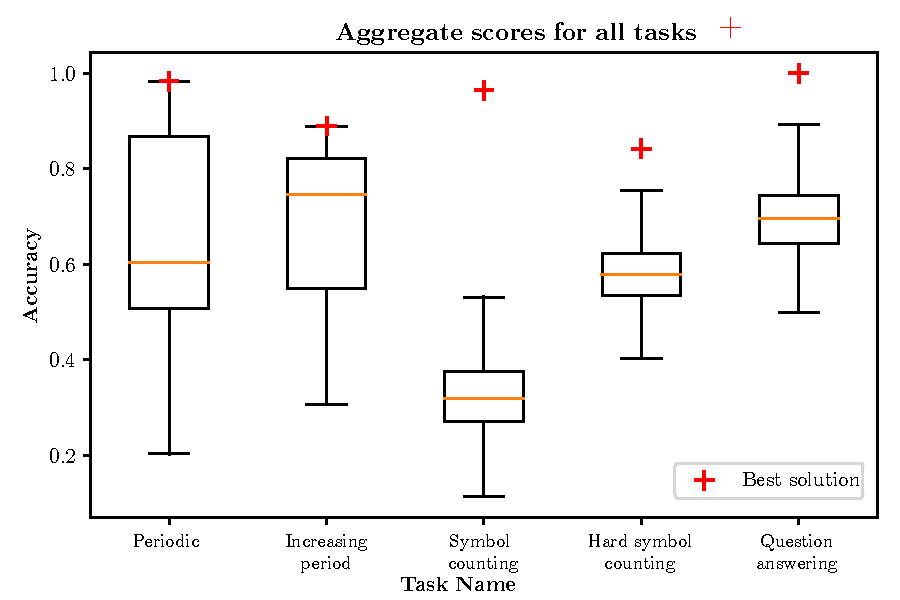
\includegraphics[width=.8\linewidth]{figures/aggregate_results.pdf}
  \caption{Average test accuracies across rules, hyperparameters, and runs for
    each task. The best solution for each task is shown in
    red.}\label{fig:aggregate-results}
\end{figure}

Fig.~\ref{fig:aggregate-results} shows a summary of the accuracy scores for each
task. Score distributions vary a lot from task to task because of the different
output spaces (binary for Periodic, Inc-per, and QA and multi-modal for the
others).

Next, we give a more in-depth analysis of the best performing \acp{ECA} on the
first two tasks.

\subsection{Binary sequences}

The binary sequence task should be the simplest to solve. Since it requires some
memory, we expect some CA rules with very chaotic behavior --- like ECA rule 30
--- to fail at it. We observed that the best rules are consistent from the
periodic and ordered types.

\begin{figure}[htbp]
  \centering
  \includegraphics[width=.7\linewidth]{figures/periodic_top.pdf}
  \caption{Top performing rules and hyperparameters for the binary periodic
    sequence task. All of the best rules seem to make use of a lateral
    translation, which is an effective memory mechanism. Rule 2, 130 and 194
    only differ by 1 transition in their rule
    function.}\label{fig:top-binary-seq}
\end{figure}

The four best rules displayed in figure \ref{fig:top-binary-seq} all implement a
a similar mechanism, using translations of cells from one column to the next at
every step. This translation is a memory mechanism because it shifts any cell
that was turned on in reaction to input before it could be overwritten by a
subsequent input that would be mapped to the same grid position.

\begin{table}[htbp]
  \centering
    \begin{tabular}{p{4cm}ccccc}
      \toprule
      & \multicolumn{5}{c}{\bfseries Top 10 rules}\\
      \midrule
      \bfseries Rule & 38 & 24 & 231 & 152 & 66 \\
      \bfseries Average accuracy & 0.969 & 0.97 & 0.97 & 0.97 & 0.97 \\
      \midrule
      \hrulefill & 189 & 194 & 52 & 130 & 2 \\
      \hrulefill & 0.97 & 0.97 & 0.97 & 0.971 & 0.971\\
      \bottomrule
    \end{tabular}
  \caption{Top 10 rules for the periodic binary sequence task (ordered left to
    right) --- best hyper-parameter combination. Many rules get close to the best
    possible accuracy.}\label{tab:top_periodic_rules}
\end{table}

\subsection{Symbol counting}

The easy version of this task yielded the most surprising results: some CA rules
unexpectedly reach very good scores. These top rules are reliably found to have
the best accuracy scores, even when using powerful decoders. The best performing
rule out of all the possible \acp{ECA} is rule 37.

\begin{figure}[htbp]
  \centering
  \includegraphics[width=\linewidth]{figures/rules-sym-ct.pdf}
  \caption{The two best performing rules for the easy symbol counting task (.82
    average accuracy).}\label{fig:best_sym_ct}
\end{figure}

As shown in figure \ref{fig:best_sym_ct}, the two best rules seem to employ a
similar ``computing mechanism'' to solve the task. They seem to grow tree-like
structures that sometimes become wider. One hypothesis for the success of these
two rules is that they encode some information about the number of observed
symbols in the width of these tree structures. \ac{RC} is useful for this kind
of analyses because it has some level of interpretability. The weights of the
output decoding layer can inform us on which of the components of the \acp{CA}
internal state are the most important for the task being solved. However, even
with this tool, it can still be hard to disentangle the effect of each
components and their interactions.

\begin{table}[htbp]
  \centering
    \begin{tabular}{p{4cm}ccccc}
      \toprule
      & \multicolumn{5}{c}{\bfseries Top 10 rules}\\
      \midrule
      \bfseries Rule & 28 & 92 & 220 & 70 & 198\\
      \bfseries Average accuracy & 0.571 & 0.572 & 0.573 & 0.574 & 0.582 \\
      \midrule
      \hrulefill & 156 & 78 & 123 & 91 & 37\\
      \hrulefill & 0.594 & 0.598 & 0.643 & 0.721 & 0.807\\
      \bottomrule
    \end{tabular}
  \caption{Top 10 rules for the easy symbol counting task (ordered left to
    right) --- best hyper-parameter combination. Notice the three best rules are
    largely better than most of the others.}\label{tab:top_sym_ct_rules}
\end{table}


\section{Conclusions}

Learning speed and data efficiency are essential components of any learning
system. Our learning speed metric can offer a novel perspective on several
machine learning models. Instead of focusing on pure performance, measuring and
comparing the data efficiency of different models will hopefully lead to better
systems for online and continual learning.


Even with the right metric, it is difficult to thoroughly evaluate a model's
ability to learn efficiently. Our benchmark evaluates a range of problem
difficulties which would be challenging to construct by combining or
manipulating existing datasets. However, the tasks remain easy to understand and
use. Since the tasks are language-based, they can be further mixed or chained to
create continual learning problems and may also be easily extended in a
follow-up work.

We study lesser-known machine learning models based on evolving states of
complex systems that can learn through self-organization. A complex dynamical
system comprises many interacting agents and evolves over time according to a
fixed update rule. These agents can be hidden neurons of a \ac{RNN} or nodes in
a graph. Such systems often exhibit emergent global dynamics resulting from the
actions of its parts rather than the decisions of a central controller. These
dynamics lead to surprisingly complex behavior, which can be random, chaotic, or
may lead to unbounded growth of complexity
\parencite{boccaraModelingComplexSystems2010}. Due to these
properties,
systems based on reservoir computing may be a promising alternative addressing
the shortcomings of standard supervised models.

Surprisingly, such models achieve remarkable learning efficiency compared to the
more standard sequential supervised models trained with stochastic
gradient-based learning. The complex systems-based models consistently
outperform sequential supervised methods and even achieve better learning
efficiency than humans on some tasks. They demonstrate more efficient learning
on our benchmark at a fraction of the computational and data cost of the
conventional models. We believe that more advanced models of this type could
lead to more robust and data efficient machine learning in the future,
especially in low-data applications or problems where supervision is limited.
Complex systems are underexplored and seem worth investigating further for
building the next generation of learning algorithms.

\chapter{Conclusion}\label{cha:conclusion}

In this chapter, we summarize our contributions in the thesis.

\section{Contributions}

In this thesis, we have developed some tools to better understand and make use
of the computations that occur within complex systems.
We summarize our contributions in the following.

\begin{itemize}
  \item In Chapter \ref{cha:background}, we gave an overview of the \acf{CA}
        model and the specific challenges it poses. We review the deep
        connection between \acp{CA} and \acfp{RNN} and how this can be used to apply
        \acp{CA} in \acf{RC}. Next, in Chapter \ref{cha:literature-review}, we
        place our work within the vast body of literature on complex systems,
        complexity, emergence, and learning.

  \item In Chapter \ref{cha:meas-compl-evolv}, we define a novel metric of
        complexity for complex systems. The metric is inspired by principles of
        compression, and algorithmic complexity. It uses the ability of small
        neural networks to learn a model of the local structures in a system,
        and the evolution of the predictive power of that model as the system
        evolves over time. We evaluated the quality of this metric by measuring
        its correlation with human perception of complexity. We find a
        higher correlation with human annotations than alternative methods on a
        dataset of \acp{CA} rules labeled as complex or not. We use the metric
        to discover new \acp{CA} rules with surprisingly complex behavior
        semi-automatically.

  \item In Chapter \ref{cha:visu-comp-large}, we built on the work of Chapter
        \ref{cha:meas-compl-evolv} to work on the specific challenges posed by
        working with large-scale systems such as cellular automata. In these
        systems, qualitatively different behavior may emerge at various scales.
        To allow dealing with these large systems and apply complexity measures
        and classification methods on a range of scales, we developed three
        coarse-graining methods based on simple statistical analysis, clustering
        algorithms and autoencoder neural networks that can reduce the size of
        a system while retaining useful information.

  \item In Chapter \ref{cha:learn-effic-compl}, we tackled the issue of using
        complex systems for general-purpose task solving, using the \ac{RC}
        paradigm. We also developed a metric for the speed of learning of
        machine learning systems. Using that metric, we looked at the data
        efficiency of some well-known algorithms rather than their task-based
        performance only. Surprisingly, \ac{RC} models using random frozen
        \acp{RNN} or \acp{CA} are significantly more efficient that other
        alternatives on a range of tasks. We evaluated this on some standard
        language datasets and introduced our own dataset of progressively more
        complex tasks. Efficiency is a crucial property in low data and compute
        settings, and our work showed that some overlooked methods may actually
        be competitive in these situations.
\end{itemize}


\setstretch{1.5}
\setlength\bibitemsep{0.5\baselineskip}
\addcontentsline{toc}{chapter}{Bibliography}
\printbibliography

\end{document}




% Structure:
%
%
% 1. Introduction (1-2 weeks)
% - Goal (picture showing the main result)
% - Motivation: why is it important (list some real applications)
    % - motivating examples
% - Challenges
%   - 
% - Contributions.
% - Thesis overview
%
% 2. Literature review (4 weeks)
% - 
% - 3 Background? (Oliver Whyte's thesis 2012 as example of Maxime Oquab) 
%
% Technical chapters. (few days to few weeks depending on what you want to do)
% -  Measuring complexity in complex systems
% -  Visualization of computation
% -  Learning efficiency of complex systems based models
% - ?? Unused material
% - Language paper??
%
% Conclusion and perspectives (1 week)
% - Contributions (2-3 pages)
% - Future work (2-3 pages)
% 
% Appendix
%
